\documentclass[11pt,a4paper,oneside]{book}
\usepackage[british,UKenglish,USenglish,english,american]{babel}
%\usepackage[a4paper, total={16cm, 23cm}]{geometry}
\usepackage[tmargin = 1.25in,bmargin = 1.25in,lmargin = 1in,rmargin = 
1in]{geometry}
\usepackage{tikz}
\usepackage{graphicx}
\usepackage{pgfplots}
\pgfplotsset{width=12cm,compat=1.9}

\usepackage{chemmacros}
\usepackage{chemfig}
%\usepackage{ghsystem}
%\usechemmodule{redox}
%\usepackage{chemnum}
%\usepackage{bohr}
%\usepackage{elements}
%\usepackage{endiagram}
%\usepackage{modiagram}
%\usepackage{chemgreek}
%\usepackage{mhchem}
\usepackage{esint}
\usepackage{tabularray}

\usepackage{makeidx}
\usepackage{epstopdf}

\usepackage{amssymb}
\usepackage{mathrsfs}
%\usepackage{minted}
\usepackage{bm}
\usepackage{amsmath}
\usepackage{enumitem}
\usepackage[english]{varioref}
\usepackage[english]{babel}
\usepackage{lipsum}
\usepackage{fancyhdr}
\pagestyle{fancy} 
\usepackage{float}
\usepackage{empheq}
\usepackage[framemethod=tikz]{mdframed}
\usepackage{epstopdf}
\numberwithin{equation}{section}
\usepackage{eso-pic}
\usepackage{calc}
\usepackage{nccmath}
\usepackage{caption}
\usepackage{subcaption}
\usepackage{gensymb}
\usepackage{amsfonts,amsthm,epsfig,epstopdf,titling,url,array}
\usepackage{siunitx}
\sisetup{input-digits = 0123456789\pi}
\usepackage[symbol]{footmisc}
\usepackage{xcolor}
\usepackage{multicol}
\usepackage{boondox-cal}
\DeclareSIUnit\atm{atm}
\setcounter{secnumdepth}{3}
\setcounter{tocdepth}{3}
\usepackage{booktabs}
\usepackage{blindtext}
\usepackage{setspace}


\DeclareSIUnit\atm{atm}

\pagestyle{fancy} 
\fancypagestyle{firstpage}{
	\rhead{\begin{picture}(0,0) 
			\put(-30,0){
\includegraphics[width=1cm]{figures/MCI_4C_bw.eps}} 
	\end{picture}}
}
\fancyhead[L]{\slshape\nouppercase{\leftmark}}
\chead{}
%\rhead{\begin{picture}(0,0) 
%		\put(-30,0){
\includegraphics[width=1cm]{figures/MCI_4C_bw.eps}} \end{picture}}
\rhead{}
\lfoot{\textit{}}
\cfoot{-\ \thepage\ -}
\rfoot{\textit{}}

\DeclareMathOperator{\rank}{rank}
\DeclareMathOperator{\atantwo}{atan2}

\def\changemargin#1#2{\list{}{\rightmargin#2\leftmargin#1}\item[]}
\let\endchangemargin=\endlist

\renewcommand{\headrulewidth}{0.4pt}
\renewcommand{\footrulewidth}{0.4pt}
\newcommand{\abs}[1]{\left|#1\right|}
\definecolor{mycolor1}{rgb}{0.97, 0.97, 0.97}
\definecolor{mycolor2}{rgb}{0.97, 0.97, 0.97}
\definecolor{tableShade}{gray}{0.9}
\newcommand{\sign}{\text{sign}}
\newcommand{\centered}[1]{\begin{tabular}{@{}l@{}} #1 \end{tabular}}
\theoremstyle{it}
\newtheorem{defn}{Definition}[chapter]
\newtheorem{assumption}{Assumption}[chapter]
\newtheorem{thm}{Theorem}[chapter]
\newtheorem{lemma}{Lemma}[chapter]
\theoremstyle{definition}
%\theoremstyle{it}
\newtheorem{example}{Example}[section]

\newenvironment{myitemize_1}
{ \begin{itemize}[topsep=0pt]
		\setlength{\topsep}{2pt}		
		\setlength{\itemsep}{2pt}
		\setlength{\parskip}{2pt}
		\setlength{\parsep}{2pt}     }
	{ \end{itemize}                  }

\newenvironment{myitemize_2}
{ \begin{itemize}[topsep=2pt]
		\setlength{\topsep}{4pt}		
		\setlength{\itemsep}{4pt}
		\setlength{\parskip}{4pt}
		\setlength{\parsep}{4pt}     }
	{ \end{itemize}                  }

\newenvironment{myitemize_3}
{ \begin{itemize}[topsep=4pt]
		\setlength{\topsep}{4pt}
		\setlength{\itemsep}{4pt}
		\setlength{\parskip}{4pt}
		\setlength{\parsep}{6pt}     }
	{ \end{itemize}                  }

\newmdenv[innerlinewidth=0.5pt, roundcorner=4pt,backgroundcolor=mycolor2, 
linecolor=mycolor1,innerleftmargin=6pt,
innerrightmargin=6pt,innertopmargin=6pt,innerbottommargin=6pt]{mybox}

\title{\textbf{ 
		\begin{LARGE}
			Induction Motor
		\end{LARGE} \\[24pt]
		\begin{Large}
			Modelization and Parameters Estimation
	\end{Large}}
}
\author{\textbf{Davide Bagnara}}

\begin{document}
	\thispagestyle{firstpage}
	\begin{mybox}
		\maketitle
		\vspace{125mm}
	\end{mybox}
	\newpage
	\tableofcontents
	\listoffigures	
	\listoftables
	\newpage

\onehalfspacing
%\setstretch{baselinestretch}
\chapter{Introduction}
The following document concerns the modelization and parameters calculation of symmetric three phase induction motors. The document starts with a description of the three phase induction motor model and proceed exploring the way how to calculate the fundamental parameters, which describe the properties of the machine, from standard factory tests.

After the exploring of the electrical machine from machine variables ($uvw$) the document introduce the use of the $\alpha\beta$ representation. This representation plays a fundamental role when a control system has to be designed. The natural extension of the $\alpha\beta$ representation, which is basically a vector representation from a fixed reference frame, is the so-called $dq$ representation where the vector description is taken from a generic rotating reference frame.  Starting from the model of the induction motor derived respect a generic reference frame, particular rotating reference frame may be adopted in order to hide or to highlight different properties.

The document proceed exploring the effects of wrong parameters estimation (in particular the rotor resistance $R_r$) and terms describing the \textit{Simscape} model developed from this document. 

\section{Nomenclature}
The following nomenclature and notation is adopted along the document:
\begin{changemargin}{0.5cm}{3cm} 
\begin{myitemize_2}
	\item[--] $\alpha\beta$ : representation respect to a stationary reference frame;	
	\item[--] $dq$ : representation respect to a reference frame rotating at to the electrical rotor speed $\omega_{r}$;	
	\item[--] $xy$ : representation respect to a reference frame rotating at to the stator rotating field $\omega_{s}$;
	\item[--] $\mathbf{x}$ : represents a generic column vector;	
	\item[--] $\mathbf{X}$ : represents a generic matrix;
	\item[--] $p$ : represents the number of poles of an electrical machine;
	\item[--] $\mathbf{f}_{uvw}^s =\begin{bmatrix} f_{su} & f_{sv} & f_{sw} \end{bmatrix}^T$ : where the term $s$ represents the stator;
	\item[--] $\mathbf{f}_{uvw}^r =\begin{bmatrix} f_{ru} & f_{rv} & f_{rw} \end{bmatrix}^T$ : where the term $r$ represents the rotor;
	\item[--] $\omega_m\quad\Big[\SI{}{\radian\per\second}\Big]$: represents the mechanical rotor speed respect to a stationary reference frame;
	\item[--] $\omega_s\quad\Big[\SI{}{\radian\per\second}\Big]$: represents the pulsation of the stator fields respect to a stationary reference frame;
	\item[--] $\omega_r=(p/2)\omega_m\quad\Big[\SI{}{\radian\per\second}\Big]$: represents the (electrical) rotor speed respect to a stationary reference frame;
	\item[--] $\vartheta_m\quad\Big[\SI{}{\radian}\Big]$: represents the mechanical rotor position (angular phase) respect to a stationary reference frame;
	\item[--] $\vartheta_r=(p/2)\vartheta_m\quad\Big[\SI{}{\radian}\Big]$: represents the (electrical) rotor position (angular phase) respect to a stationary reference frame;
	\item[--] $\omega_0\quad\Big[\SI{}{\radian\per\second}\Big]$: represents the rotational speed of a generic rotating reference frame;
	\item[--] $n\quad\Big[\SI{}{\per\minute}\Big]$: represents the mechanical rotor speed in \textit{rpm} (revolution per minute);
	\item[--] $n_s\quad\Big[\SI{}{\per\minute}\Big]$: represents the synchronous (no-load speed) mechanical rotor speed in \textit{rpm} (revolution per minute);
	\item[--] $s$: represents the slip, and is defined as $s=(n_s - n)/n_s$, and is measured in per unit;
	\item[--] $x_{nl}$: a variable or parameter which concerns with the no-load test;
	\item[--] $x_{br}$: a variable or parameter which concerns with the blocked-rotor test.
\end{myitemize_2}
\end{changemargin}



\chapter{Symmetrical Induction Machines}
\section{Voltage equations in machine variables}\label{voltage_equations_in_machine_variables}
The voltage equations in machine variables may be expressed as follows
\begin{flalign}
	\mathbf{u}_{uvw}^s &= \mathbf{R}_s\mathbf{i}_{uvw}^s + \frac{d}{dt}\mathbf{\psi}_{uvw}^s \label{im_krause_eq1}\\[6pt]
	\mathbf{u}_{uvw}^r &= \mathbf{R}_r\mathbf{i}_{uvw}^r + \frac{d}{dt}\mathbf{\psi}_{uvw}^r \label{im_krause_eq2}
\end{flalign}
where 
\begin{flalign}
	\mathbf{f}_{uvw}^s&=\begin{bmatrix} f_{su} & f_{sv} & f_{sw} \end{bmatrix}^T \\[6pt]
	\mathbf{f}_{uvw}^r&=\begin{bmatrix} f_{ru} & f_{rv} & f_{rw} \end{bmatrix}^T
\end{flalign}
where $s$ denotes variables and parameters associated with the stator circuits, and $r$ denotes variables and parameters associated with the rotor circuits. Both $\mathbf{R}_s$ and $\mathbf{R}_r$ are diagonal matrices each with equal nonzero elements. For magnetically linear system, the flux linkages may be described as
\begin{equation}\label{im_krause_eq3}
	\begin{bmatrix} \mathbf{\psi}_{uvw}^s \\[6pt] \mathbf{\psi}_{uvw}^r \end{bmatrix} = \begin{bmatrix} \mathbf{L}_s & \mathbf{L}_{sr} \\[6pt] (\mathbf{L}_{sr})^T & \mathbf{L}_r\end{bmatrix}\begin{bmatrix} \mathbf{i}_{uvw}^s \\[6pt] \mathbf{i}_{uvw}^r \end{bmatrix}
\end{equation}
Neglecting mutual leakage between the stator windings and also between the rotor windings, the winding inductances may be expressed as follows
\begin{equation}\label{im_krause_eq4}
	\mathbf{L}_{s} = \begin{bmatrix} L_s & -\frac{1}{2}L_{sm} & -\frac{1}{2}L_{sm} \\[6pt] -\frac{1}{2}L_{sm} & L_s & -\frac{1}{2}L_{sm} \\[6pt] -\frac{1}{2}L_{sm} & -\frac{1}{2}L_{sm} & L_s \end{bmatrix}
\end{equation}
where $L_s=L_{sd}+L_{sm}$.
\begin{equation}\label{im_krause_eq5}
	\mathbf{L}_{r} = \begin{bmatrix} L_r & -\frac{1}{2}L_{rm} & -\frac{1}{2}L_{rm} \\[6pt] -\frac{1}{2}L_{rm} & L_r & -\frac{1}{2}L_{rm} \\[6pt] -\frac{1}{2}L_{rm} & -\frac{1}{2}L_{rm} & L_r \end{bmatrix}
\end{equation}
where $L_r=L_{rd}+L_{rm}$.
\begin{equation}\label{im_krause_eq6}
	\mathbf{L}_{sr} = {L}_{sm}\begin{bmatrix} \cos(\theta_r) & \cos(\theta_r+\frac{2\pi}{3}) & \cos(\theta_r-\frac{2\pi}{3}) \\[6pt] \cos(\theta_r-\frac{2\pi}{3}) & \cos(\theta_r) & \cos(\theta_r+\frac{2\pi}{3}) \\[6pt] \cos(\theta_r+\frac{2\pi}{3}) & \cos(\theta_r-\frac{2\pi}{3}) & \cos(\theta_r) \end{bmatrix}
\end{equation}
where 
\begin{flalign}
	L_{sm}=L_{rm}=L_m \label{im_krause_eq7}
\end{flalign}

In Eqs.~\eqref{im_krause_eq4}--~\eqref{im_krause_eq6} $L_s$ and $L_{sm}$ are, respectively, the leakage and magnetizing inductances of the stator windings; $L_r$ and $L_{rm}$ are for rotor windings. The inductance $L_{sm}$ is the amplitude of the mutual inductances between stator and rotor windings.

It is important to remark, that, it is assumed that the induction machine is a linear (no saturation) and the \textit{mmf} (magneto-motive force) are harmonic-free device.

The voltage equations expressed in terms of machine variables referred to the stator windings may be written as follows
\begin{flalign}
	\mathbf{u}_{uvw}^s &= \mathbf{R}_s\mathbf{i}_{uvw}^s + \frac{d}{dt}\Big(\mathbf{L}_s\mathbf{i}_{uvw}^s\Big) + \frac{d}{dt}\Big(\mathbf{L}_{sr}\mathbf{i}_{uvw}^r\Big) \label{im_krause_eq8} \\[6pt]
	\mathbf{u}_{uvw}^r &= \mathbf{R}_r\mathbf{i}_{uvw}^r + \frac{d}{dt}\Big(\mathbf{L}_r\mathbf{i}_{uvw}^r\Big) + \frac{d}{dt}\Big[\big(\mathbf{L}_{sr}\big)^T\mathbf{i}_{uvw}^s\Big] \label{im_krause_eq9}
\end{flalign}

\section{Torque equation in machine variables}
The energy stored in the coupling field may be written as follows
\begin{flalign}
	W_f = \frac{1}{2}\big(\mathbf{i}_{uvw}^s\big)^T\mathbf{L}_s\mathbf{i}_{uvw}^s + \big(\mathbf{i}_{uvw}^s\big)^T\mathbf{L}_{sr}\mathbf{i}_{uvw}^r + \frac{1}{2}\big(\mathbf{i}_{uvw}^r\big)^T\mathbf{L}_r\mathbf{i}_{uvw}^r \label{im_krause_eq10}
\end{flalign}
Since the machine is assumed to be magnetically linear, the field energy $W_f$ is equal to the coenergy $W_c$.

The change of mechanical energy in a rotational system with one mechanical input may be written as follows
\begin{flalign}
	dW_m = -\tau_{e}d\vartheta_{m} \label{im_krause_eq11}
\end{flalign}
where $\tau_{e}$ is the electromagnetic torque and $\vartheta_{m}$ is the mechanical rotor displacement. Since
\begin{flalign}
	\vartheta_{r}=\frac{p}{2}\vartheta_{m} \label{im_krause_eq12}
\end{flalign}
where $p$ is the number of poles in the machine, then
\begin{flalign}
	dW_m = -\tau_{e}\frac{2}{p}d\vartheta_{r} \label{im_krause_eq13}
\end{flalign}
Therefore, the electromagnetic torque may be derived from the equation
\begin{flalign}
	\tau_{e}(\mathbf{i},\vartheta_{r})=\frac{p}{2}\frac{\partial W_c(\mathbf{i},\vartheta_{r})}{\partial \vartheta_{r}} \label{im_krause_eq14}
\end{flalign}
Since $\mathbf{L}_s$ and $\mathbf{L}_r$ are not function of $\vartheta_{r}$, substituting $W_f$ from \eqref{im_krause_eq10} into \eqref{im_krause_eq14} yields the electromagnetic torque in \SI{}{\newton\meter}
\begin{flalign}
	\tau_{e} = \frac{p}{2}\big(\mathbf{i}_{uvw}^s\big)^T
	\Bigg(\frac{\partial}{\partial \vartheta_{r}}\mathbf{L}_{sr}\Bigg)
	\mathbf{i}_{uvw}^r \label{im_krause_eq15}
\end{flalign}
which become
\begin{equation}\label{im_krause_eq16}
	\begin{aligned}
			\tau_{e} = &-\frac{p}{2}L_m\Bigl\{\Bigl[i_{su}\Big(i_{ru}-\frac{1}{2}i_{rv}-\frac{1}{2}i_{rw}\Big) + 
		i_{sv}\Big(i_{rv}-\frac{1}{2}i_{ru}-\frac{1}{2}i_{rw}\Big) \\[8pt]
		& + i_{sw}\Big(i_{rw}-\frac{1}{2}i_{rv}-\frac{1}{2}i_{ru}\Big)\Bigr]\sin\vartheta_r
		+ \frac{\sqrt{3}}{2}\Big[i_{su}\Big(i_{rv}-i_{rw}\Big) \\[8pt]
		& + i_{sv}\Big(i_{rw}-i_{ru}\Big) + i_{sw}\Big(i_{ru}-i_{rv}\Big)\Big]\cos\vartheta_{r}
		\Bigr\} 
	\end{aligned}
\end{equation}
The torque and speed are related by the equation
\begin{flalign}
	\tau_{e} = J\frac{2}{p}\frac{d}{dt}\omega_{r} + \tau_l \label{im_krause_eq17}
\end{flalign}
where $J$ is the inertia of the rotor and in some cases the connected load, $\tau_l$ is the load torque.


\chapter{Steady State Analysis of the Induction Motor}

\section{Equivalent Circuit}
Let us assume that the rotor is turning at the steady speed of $n$ [\SI{}{\per\minute}] in the same direction as the rotating stator field. Let the synchronous speed of the stator field be $n_s$ [\SI{}{\per\minute}]. The difference between synchronous speed and the rotor speed is the slip $n_s-n$, and may be used to define the slip factor. The slip factor is defined as as slip as fraction of the synchronous speed, namely
\begin{equation} \label{eq1}
	s=\frac{n_s - n}{n_s}
\end{equation}
with the properties to be independent from the unity of measure, in fact the slip factor $s$ is defined in per unit.

Similarly, the mechanical angular velocity $\omega_m$ may be expressed in terms of the synchronous angular velocity $\omega_s$ and slip factor as follows
\begin{equation} \label{eq2}
	\omega_r=(1-s)\omega_s
\end{equation}
The relative motion of the stator flux and the rotor conductors induces voltages of pulsation $\omega_{sl}$ respect to a rotating reference frame at to the rotor speed $\omega_r$
\begin{flalign} 
	\omega_{sl} &= s\omega_s \label{eq3a}
%	\omega_{s} &= \omega_{sl} + \omega_r \label{eq3b}
\end{flalign}
the $\omega_{sl}$ is referred to as the \textit{slip pulsation} in the rotor.

With the rotor revolving in the same direction of the rotation as the stator field, the pulsation of the rotor currents will be $\omega_{sl}$ and they will produce a rotating flux wave which will rotate at $\omega_{sl}$, respect to a rotating reference frame at to the rotor speed $\omega_r$, and in the forward direction. Thus, with respect to the stator, the rotor speed and the flux wave produced by the rotor currents is the sum of these two speeds and equals
\begin{flalign} 
	\omega_{s} &= \omega_{sl} + \omega_r \label{eq4}
\end{flalign}
From Eq.~\eqref{eq4} we see that the rotor currents produce an air-gap flux wave which rotates at synchronous speed (respect to a fixed reference frame) and hence is synchronous with the flux produced by the stator currents. Because the stator and rotor fields each rotate \textbf{synchronously}, the are stationary with respect to each other and produce a steady torque.

In the range of small slip factor, from 2 to 10 percent, torque is \textbf{proportional} with slip factor, moreover, the value of slip factor at which the peak torque occurs is proportional to the rotor resistance.

The foregoing considerations of flux and \textit{mmf} waves may be translated to a steady state equivalent circuit.

The equivalent circuit is built supposing the three phase machine as being Y-connected, so that currents are always line values and voltages always line to neutral values.
The synchronous rotating air-gap flux wave generates balanced polyphase back \textit{emfs} in the phases of the stator. The stator terminal voltage differs from the back \textit{emf} by the voltage drop in the stator leakage impedance $Z_1 = R_s + jX_{d1}$. Thus
\begin{equation} \label{eq5}
	V_1 = E_2 + I_1 (R_s + jX_{d1})
\end{equation}
where
\begin{itemize}
	\item[--] $V_1$ : Stator line-to-neutral terminal voltage phasor\footnote{ Consider a sinusoidal signal of the form
	\begin{flalign}
		a(t)=A\cos(\omega t+\phi)=\Re\Big(Ae^{j\phi}e^{j\omega t}\Big)
	\end{flalign}
the term $Ae^{j\phi}$ represents the phasor of the signal $a(t)$. All mathematics of iso-frequency signals may be performed using the phasors of the form $Ae^{j\phi}$ where pulsation is implied.};
	\item[--] $E_2$ : Back \textit{emf} (line-to-neutral) phasor generated by the resultant air-gap flux;
	\item[--] $I_1$ : Stator current phasor;
	\item[--] $R_s$ : Stator effective resistance;
	\item[--] $X_{d1}$ : Stator leakage reactance;
\end{itemize}
\begin{figure}[H]
	\centering
	\includegraphics[width = 225pt, keepaspectratio]{figures/stator_equivalent_circuit.eps}
	\captionsetup{width=0.5\textwidth, font=small}		
	\caption{Stator equivalent circuit.}
	\label{stator_equivalent_circuit} 
\end{figure}
The resulting air-gap flux is created by combined \textit{mmfs} of the stator and rotor currents. The load component $I_2$ produces an \textit{mmf} that corresponds to the \textit{mmf} of the rotor currents. The exciting component $I_{\varphi}$ is the additional stator current required to create the resultant air-gap flux and is a function of the back \textit{emf} $E_2$.
From the point of view of the stator equivalent circuit, the rotor may be represented by an equivalent impedance $Z_2$
\begin{equation} \label{eq6}
	Z_2 = \frac{E_2}{I_2}
\end{equation}
To complete the equivalent circuit, we must determine $Z_2$ by representing the stator and rotor voltages and currents in terms of rotor quantities as referred to the stator.

Let $E_{2s}$ be the voltage induced in the equivalent rotor by the resultant air-gap flux, and $I_{2s}$ be the corresponding induced current, consequently the slip-frequency ($\omega_{sl}$) leakage impedance $Z_{2s}$ is given by
\begin{equation} \label{eq7}
	Z_{2s} = \frac{E_{2s}}{I_{2s}} = R_r+jsX_{d2}
\end{equation}
where
\begin{itemize}
	\item[--] $R_r$ : rotor resistance	
	\item[--] $sX_{d2}$ : rotor leakage reactance at slip pulsation $\omega_{sl}$
	\item[--] $X_{d2}$ : rotor leakage reactance at stator pulsation $\omega_s$
\end{itemize}	
\begin{figure}[H]
	\centering
	\includegraphics[width = 150pt, keepaspectratio]{figures/rotor_equivalent_circuit.eps}
	\captionsetup{width=0.5\textwidth, font=small}		
	\caption{Rotor equivalent circuit at slip frequency~($\omega_{sl}$).}
	\label{rotor_equivalent_circuit} 
\end{figure}
By the assumption of the same number of turns per phase of stator and rotor, $I_2$ and $I_{2s}$ must be equal in magnitude and phase (at their respective electrical frequencies) and hence we may write\footnote{$I_{2s}$ pulsation corresponds to $\omega_{sl}=s\omega_{s}$, while $I_{2}$ pulsation corresponds to $\omega_{s}$. Eq.~\eqref{eq8} says that the \textbf{phasors} $I_{2s}$ and $I_{2}$ are equal in phase and in magnitude, but not in pulsation.}
\begin{equation} \label{eq8}
	I_{2s} = I_{2}
\end{equation}
and
\begin{equation} \label{eq9}
	E_{2s} = sE_{2}
\end{equation}
from which
\begin{equation} \label{eq10}
	\frac{E_{2s}}{I_{2s}}=\frac{sE_2}{I_2}=Z_{2s}=R_r+jsX_{d2}
\end{equation}
\begin{equation} \label{eq11}
	Z_{2}=\frac{E_2}{I_2}=\frac{R_r}{s}+jX_{d2}=R_r+jX_{d2}+R_r\frac{1-s}{s}
\end{equation}
The single phase equivalent circuit of Fig. \ref{equivalent_circuit} may be used to determine a wide variety of steady-state performance characteristics of polyphase induction machines. The equivalent circuit shows that the total power $P_{gap}$ transferred across the air gap from the stator is
\begin{equation} \label{eq12}
	P_{gap}= q I_2^2 \left( \frac{R_r}{s} \right)
\end{equation}
where q is the number of the phases.
\begin{figure}[H]
	\centering
	\includegraphics[width = 275pt, keepaspectratio]{figures/equivalent_circuit.eps}
	\captionsetup{width=0.5\textwidth, font=small}		
	\caption{IM equivalent circuit.}
	\label{equivalent_circuit} 
\end{figure}
The total rotor $I^2R$ losses, $P_{rotor}$, may be calculated from the $I^2R$ losses in the equivalent rotor as
\begin{equation} \label{eq13}
	P_{rotor}= q I_{2s}^2 R_r
\end{equation}
Since $I_{2s}=I_2$, we may write 
\begin{equation} \label{eq14}
	P_{rotor}= q I_{2}^2 R_r
\end{equation}
The electromechanical power $P_{mech}$ developed by the motor may be determined by subtracting the rotor power dissipation from the air-gap power.
\begin{equation} \label{eq15}
	P_{mech} = P_{gap} - P_{rotor} = q I_{2}^2 \left( \frac{R_r}{s} \right) - q I_{2}^2 R_r
\end{equation} 
or equivalently
\begin{equation} \label{eq16}
	P_{mech} = q I_{2}^2 R_r \left( \frac{1-s}{s} \right)
\end{equation} 
The electromechanical torque $T_{mech}$ corresponding to the power $P_{mech}$ may be obtained by recalling that mechanical power equals torque times angular velocity. Thus\footnote{$p$ represents the number of poles.},
\begin{equation} \label{eq17}
	T_{mech} = \left(\frac{p}{2\omega_e} \right) q I_{2}^2 \left( \frac{R_r}{s} \right)
\end{equation} 

\chapter{Induction Motor Parameter Calculation}
The equivalent circuit parameters needed for computing the performance of the poly-phase induction motor under load may be obtained from the results of a no-load test, a blocked-rotor test and measurements of the dc resistances of the stator windings. For a complete determination of the parameters, both reactive power $Q_{nl}$, $Q_{br}$ and active power $P_{nl}$, $P_{br}$ shall be measured, but often these information are available in partial way and additional information are necessary. The nominal load test is in general very useful to complete the calculation of the equivalent circuit, in fact this test reports clearly the correlation between nominal torque and nominal slip which is the fundamental parameter to calculate the rotor resistance by the mean of the equivalent circuit. Thus, the following tests may be assumed necessary to calculate the parameters of the equivalent electrical circuit of the induction motor. 
\begin{changemargin}{0.5cm}{3cm} 
	\begin{myitemize_2}
	\item[--] DC-measure of the winding resistance.
	\item[--] No-load test: calculation of the $L_s = L_{sd} + L_m$.
	\item[--] Blocked-rotor test: calculation of $L_{\sigma}$ where $L_{rd}=L_{sd}=\frac{1}{2}L_{\sigma}$.
	\item[--] Nominal load test: calculation of the $R_r$ with a iterative process using the equivalent circuit set with a initial value of the $R_r = R_r^{preset}$.
	\end{myitemize_2}
\end{changemargin}

\section{No-load test}
Noting that the no-load power factor is very small (i.e. $Q_{nl} \gg P_{nl}$) and hence $R_s \ll (X_{d1}+X_m)$, the no-load reactance may often be approximated to (see also Figure~\ref{no_load_test})
\begin{equation} \label{eq18}
	X_{nl} \approx \frac{V_{1,nl}}{I_{1,nl}}
\end{equation} 
That means by the knowledge of the no-load test, the magnetization current and the first estimation of the magnetization inductance may be determined. The knowledge of the magnetization current magnitude remains a fundamental parameter for the control system design and implementation.
\begin{figure}[H]
	\centering
	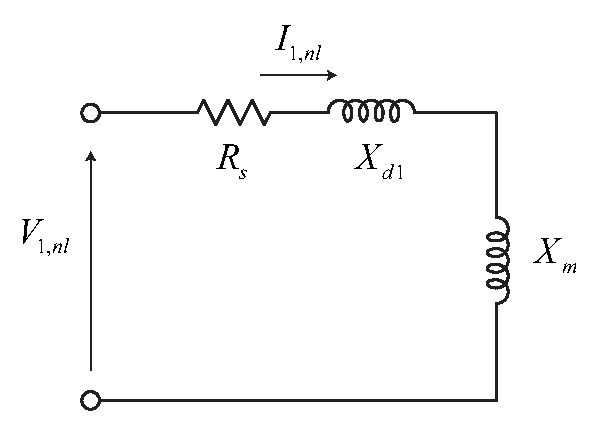
\includegraphics[width = 175pt, keepaspectratio]{figures/no_load_test.eps}
	\captionsetup{width=0.5\textwidth, font=small}
	\caption{Approximate induction motor equivalent circuit: no-load conditions.}
	\label{no_load_test} 
\end{figure}


\section{Blocked-rotor test}
Blocked-rotor test is used to calculate the $L_{d2}$ leakage inductance even if, theoretically, may be used to calculate the rotor resistance $R_r$. 
In the following we will show the complete calculation of the parameters using the locked-rotor test. After that,  the nominal load test will be used to finally correct and identify the rotor resistance, in fact, the effective slip at nominal load gives the correct information for the calculation of the motor torque, namely, of the rotor resistance. The value of the actual slip and the value of the actual torque are strictly related to the value of the rotor resistance.
\begin{figure}[H]
	\centering
	\includegraphics[width = 275pt, keepaspectratio]{figures/rotor_res_effects_2.eps}
	\captionsetup{width=0.5\textwidth, font=small}		
	\caption{Induction motor torque slip curves showing effect of changing rotor circuit resistance.}
	\label{rotor_res_effects} 
\end{figure}
Based upon blocked-rotor measurement, the blocked-rotor reactance may be found from the blocked-rotor reactive power (see also Figure~\ref{rotor_locked_test})
\begin{equation} \label{eq19}
	Q_{bl} = \sqrt{S_{br}^2+P_{br}^2}
\end{equation} 
The blocked rotor reactance, corrected to the rated frequency (sometimes the blocked rotor test is executed at different frequency)
\begin{equation} \label{eq20}
	X_{br} = \left( \frac{f_{re}}{f_{br}}\right) \left(\frac{Q_{br}}{qI_{1,br}^2}\right)
\end{equation} 
The blocked-rotor resistance may be calculated from the blocked-rotor input power as 
\begin{equation} \label{eq21}
	R_{br} = \frac{P_{br}}{qI_{1,br}^2}
\end{equation} 
Once these parameters have been determined, the equivalent circuit parameters can be determined. Under blocked~-~rotor conditions, an expression for the stator input impedance may be obtained from the examination of Figure~\ref{rotor_locked_test}
\begin{equation} \label{eq22}
	\begin{aligned}
		Z_{br} 	= & R_s + jX_{d1} + \left( R_r + j X_{d2} \right) \textmd{ in parallel with } jX_m \\[6pt]
		= & R_s + \frac{R_rX_m^2}{R_r^2+(X_m+X_{d2})^2} \\[6pt]
		& + j \left(X_{d1} + \frac{X_m(R_r^2+X_{d2}(X_m+X_{d2}))}{R_r^2+(X_m+X_{d2})^2}\right)
	\end{aligned}
\end{equation}
Hence the corresponding blocked-rotor resistance is thus given by
\begin{equation} \label{eq23}
	R_{br} = R_s + \frac{R_rX_m^2}{R_r^2+(X_m+X_{d2})^2} 
\end{equation} 
and the the corresponding blocked-rotor reactance is
\begin{equation} \label{eq24}
	X_{br} = X_{d1} + \frac{X_m(R_r^2+X_{d2}(X_m+X_{d2}))}{R_r^2+(X_m+X_{d2})^2}
\end{equation} 
\begin{figure}[H]
	\centering
	\includegraphics[width = 250pt, keepaspectratio]{figures/rotor_locked_test.eps}
	\captionsetup{width=0.5\textwidth, font=small}		
	\caption{Induction motor equivalent circuit: blocked-rotor conditions.}
	\label{rotor_locked_test} 
\end{figure}
Due to condition of $R_r \ll X_m$ equations \eqref{eq23} and \eqref{eq24} may be reduced to
\begin{equation} \label{eq25}
	R_{br} = R_s + R_r \left(\frac{X_m}{X_m+X_{d2}}\right)^2
\end{equation} 
and 
\begin{equation} \label{eq26}
	X_{br} = X_{d1} + X_{d2} \left( \frac{X_m}{X_m+X_{d2}} \right)
\end{equation}
From the above equations the rotor resistance and leakage reactance can be found as follows
\begin{equation} \label{eq27}
	R_{r} = \left(R_{br} - R_{s} \right) \left( \frac{X_m+X_{d2}}{X_m} \right)^2
\end{equation}
The performance of the motor is affected relatively little by the way in which the total leakage reactance is distributed between the stator and rotor and in general is taken as $X_{d1} = X_{d2}$
\begin{equation} \label{eq27}
	\left\{
	\begin{aligned} 
		X_{d2} = & \left(X_{br} - X_{d1}\right) \left( \frac{X_m}{X_m+X_{d1}-X_{br}} \right) \\[6pt]
		X_{m} =  & X_{nl} - X_{d1}
	\end{aligned}\right.
\end{equation}


\subsection{Rotor resistance from steady state nominal load test}
The calculation of the rotor resistance from steady state nominal load condition is performed via equivalent circuit, by the measure of the following test data:
\begin{itemize}
	\item voltage input;
	\item current input;
	\item input power or shaft torque;
	\item stator frequency;
	\item rotor speed.
\end{itemize}
From equivalent circuit of the induction motor, where all data are already calculated from the dc-measure of the stator winding, no-load test and locked-rotor test, the $I_2$ current is calculated with a preliminary underestimate value of $R_r(0)$. Now, iteratively, for each step a small $\Delta R_r$ is add to the initial value of $R_r(k)=\Delta R_r+R_r(k-1)$ and the relative torque (as seen in Eq.~\eqref{eq17}) is calculated. The iteration stops when for a given $R_r(n)$ the nominal torque value is reached. The value of $R_r(n)$, which gives the nominal value of torque, completes the calculation of the parameters of the equivalent circuit.

\chapter{Reference-Frame Theory}
Some of the machine inductances are functions of the rotor position, whereupon the coefficients of the differential equations that describe the behaviour of these machines are rotor position dependent. A change of variables is often used to reduce the complexity of these differential equations.

\section{Change of variables}
Although changes of variables are used in the analysis of ac machines to eliminate time-varying inductances, changes of variables are also employed in the analysis of various static, constant-parameter power-system components and control systems associated with electrical drives.

A change of variables that formulates a transformation of the three-phase variables of stationary circuit elements to the arbitrary reference frame may be expressed as
\begin{flalign}
	\mathbf{f}_{qd0}^s=\mathbf{K}_s\mathbf{f}_{uvw}^s \label{RFT_eq1}
\end{flalign}
where 
\begin{flalign}
	\big(\mathbf{f}_{qd0}^s\big)^T &= \begin{bmatrix} f_{qs} & f_{ds} & f_{0s}\end{bmatrix} \label{RFT_eq2} \\[6pt]
	\big(\mathbf{f}_{uvw}^s\big)^T &= \begin{bmatrix} f_{us} & f_{vs} & f_{ws}\end{bmatrix} \label{RFT_eq3} \\[6pt]
	\mathbf{K}_{s} &= \frac{2}{3}\begin{bmatrix} \cos\vartheta & \cos\big(\vartheta-\frac{2\pi}{3}\big) & \cos\big(\vartheta+\frac{2\pi}{3}\big) \\[6pt] \sin\vartheta & \sin\big(\vartheta-\frac{2\pi}{3}\big) & \sin\big(\vartheta+\frac{2\pi}{3}\big) \\[6pt] \frac{1}{2} & \frac{1}{2} & \frac{1}{2} \end{bmatrix} \label{RFT_eq4} 
\end{flalign}
where the angular position and velocity of the arbitrary reference frame are related as follows
\begin{flalign}
	\frac{d\vartheta}{dt}=\omega \label{RFT_eq5} 
\end{flalign}
It can be shown that the inverse transformation is
\begin{flalign}
	\big(\mathbf{K}_{s}\big)^{-1} &= \begin{bmatrix} \cos\vartheta & \sin\vartheta & 1 \\[6pt] \cos\big(\vartheta-\frac{2\pi}{3}\big) & \sin\big(\vartheta-\frac{2\pi}{3}\big) & 1 \\[6pt] \cos\big(\vartheta+\frac{2\pi}{3}\big) & \sin\big(\vartheta+\frac{2\pi}{3}\big) & 1 \end{bmatrix} \label{RFT_eq6} 
\end{flalign}
In the above equations, $f$ may represent either voltage, current, flux linkage, or electric charge. The superscript $T$ denotes the transpose of a matrix, The $s$ subscript indicates the variables, parameters, and transformation associated with stationary circuits, The angular displacement $\vartheta$ must be continuous; however, the angular velocity associated with the change of variables is unspecified. The frame of reference may rotate at any constant or varying angular velocity. The connotation of arbitrary stems from the fact that the angular velocity of the transformation is unspecified and may be selected arbitrarily to expedite the solution of the system equations or to satisfy the system constraints. 

The total instantaneous power of a three-phase system may be expressed in $uvw$ variables as follows
\begin{flalign}
	P_{uvw}^s=v_{us}i_{us}+v_{vs}i_{vs}+v_{ws}i_{ws} \label{RFT_eq7} 
\end{flalign}
The total power expressed in the $qd0$ variables must equals to the total power expressed in the $uvw$ variables, hence, using \eqref{RFT_eq1} to replace actual currents and voltages in \eqref{RFT_eq7} yields
\begin{flalign}
	P_{qd0}^s=P_{uvw}^s=\frac{3}{2}\Big(v_{qs}i_{qs}+v_{ds}i_{ds}+2v_{0s}i_{0s}\Big) \label{RFT_eq8} 
\end{flalign}
Although the waveforms of the $qs$ and $ds$ voltages, currents, flux linkages, and electrical charges are dependent upon the angular velocity of the frame of reference, the waveform of the total power is the same regardless of the reference frame in which it is evaluated.

\vspace{5mm}\textbf{For a three-phase resistive circuit}
\begin{flalign}
	\mathbf{v}_{uvw}^s=\mathbf{R}_s\mathbf{i}_{uvw}^s \label{RFT_eq9}
\end{flalign} 
From \eqref{RFT_eq1} 
\begin{flalign}
	\mathbf{v}_{qd0}^s=\mathbf{K}_s\mathbf{R}_s\Big(\mathbf{K}_s\Big)^{-1}\mathbf{i}_{qd0}^s \label{RFT_eq10}
\end{flalign} 
Power systems are always made in a way to obtain equal distributed load around the phases, namely, the matrix $\mathbf{R}$ is a diagonal matrix with identical elements $\mathbf{R}=\text{diag}\begin{bmatrix} R_{us} & R_{vs} & R_{ws} \end{bmatrix}$ with $R_{xs}=R_s$.  
That means
\begin{flalign}
	\mathbf{K}_s\mathbf{R}_s\Big(\mathbf{K}_s\Big)^{-1} = \mathbf{R}_s \label{RFT_eq11}
\end{flalign} 
Thus, the resistance matrix associated with the arbitrary reference variables $\big(f_{qs},\ f_{ds},\ f_{0s}\big)$ is equal to the resistance matrix associated with the actual variables if each phase of the actual circuit has the same resistance, $R_{xs}=R_s$. If the phase resistances are unequal (unbalanced or unsymmetrical), then the resistance matrix associated with the arbitrary reference-frame variables contains sinusoidal functions of $\vartheta$ except when $\omega=0$, whereupon $\mathbf{K}_s$ is algebraic. In other words, if the phase resistances are unbalanced, the transformation yields constant resistance only if the reference frame is fixed where the unbalance physically exists. 

\vspace{5mm}\textbf{For a three-phase inductive circuit}
\begin{flalign}
	\mathbf{v}_{uvw}^s= \frac{d}{dt}\boldsymbol{\psi}_{uvw}^s\label{RFT_eq12}
\end{flalign} 
In the case of the magnetically linear system, it has been customary to express the flux linkages as a product of inductance and current matrices before performing a change of variables. However, the transformation is valid for flux linkages and an extensive amount of work can be avoided by transforming the flux linkage directly. This is especially true in the analysis of ac machines, where the inductance matrix is a function of rotor position. Thus, in terms of the substitute variables, \eqref{RFT_eq12} become
\begin{flalign}
	\mathbf{v}_{qd0}^s= \mathbf{K}_s\frac{d}{dt}\Big[\Big(\mathbf{K}_s\Big)^{-1}\boldsymbol{\psi}_{qd0}^s\Big] \label{RFT_eq13}
\end{flalign} 
which can be written as
\begin{flalign}
	\mathbf{v}_{qd0}^s= \mathbf{K}_s\frac{d}{dt}\Big[\Big(\mathbf{K}_s\Big)^{-1}\Big]\boldsymbol{\psi}_{qd0}^s +\frac{d}{dt}\boldsymbol{\psi}_{qd0}^s \label{RFT_eq14}
\end{flalign} 
It is easy to show that
\begin{flalign}
	\frac{d}{dt}\Big[\Big(\mathbf{K}_s\Big)^{-1}\Big]=\omega\begin{bmatrix}
		-\sin\vartheta & \cos\vartheta & 0 \\[6pt]
		-\sin\big(\vartheta-\frac{2\pi}{3}\big) & \cos\big(\vartheta-\frac{2\pi}{3}\big) & 0 \\[6pt]
		-\sin\big(\vartheta+\frac{2\pi}{3}\big) & \cos\big(\vartheta+\frac{2\pi}{3}\big) & 0
	\end{bmatrix} \label{RFT_eq15}
\end{flalign} 
Therefore
\begin{flalign}
	\mathbf{K}_s\frac{d}{dt}\Big[\Big(\mathbf{K}_s\Big)^{-1}\Big]=\omega\begin{bmatrix}
		0 & 1 & 0 \\[6pt]
		-1 & 0 & 0 \\[6pt]
		0 & 0 & 0
	\end{bmatrix} \label{RFT_eq16}
\end{flalign} 
Equation~\eqref{RFT_eq14} may be expressed as
\begin{flalign}
	\mathbf{v}_{qd0}^s= \omega\begin{bmatrix}
		0 & 1 & 0 \\[6pt]
		-1 & 0 & 0 \\[6pt]
		0 & 0 & 0
	\end{bmatrix}\boldsymbol{\psi}_{qd0}^s+\frac{d}{dt}\boldsymbol{\psi}_{qd0}^s \label{RFT_eq17}
\end{flalign} 
In expanded form become
\begin{flalign}
	v_{qs} &= \omega\psi_{ds}+\frac{d}{dt}\psi_{qs}\label{RFT_eq18} \\[6pt]
	v_{ds} &= -\omega\psi_{qs}+\frac{d}{dt}\psi_{ds}\label{RFT_eq19} \\[6pt]
	v_{0s} &= \frac{d}{dt}\psi_{0s}\label{RFT_eq20}
\end{flalign} 
The first term on the right side of \eqref{RFT_eq18} or \eqref{RFT_eq19} is referred to as a ``speed voltage'', with the speed being the angular velocity of the arbitrary reference frame. It is clear that the speed voltage terms are zero if $\omega$ is zero,  which, of course, is when the reference frame is stationary. Clearly, the voltage equations for the three-phase inductive circuit become the familiar time rate of change of flux linkages if the reference frame is fixed where the circuit physically exists, 

For a linear system, the flux linkages may be expressed
\begin{flalign}
	\boldsymbol{\psi}_{uvw}^s=\mathbf{L}_s\mathbf{i}_{uvw}^s \label{RFT_eq21}
\end{flalign} 
Whereupon, the flux linkages in the arbitrary reference frame may be written as
\begin{flalign}
	\boldsymbol{\psi}_{qd0}^s=\mathbf{K}_s\mathbf{L}_s\big(\mathbf{K}_s\big)^{-1}\mathbf{i}_{qd0}^s \label{RFT_eq22}
\end{flalign} 
As in the case of the resistive circuit, it is necessary to specify the inductance matrix before proceeding with the evaluation of \eqref{RFT_eq22}. However, once the inductance matrix is specified, the procedure for expressing any three-phase inductive circuit in the arbitrary reference frame reduces to one of evaluating \eqref{RFT_eq22} and substituting the resulting $\psi_{qs}$, $\psi_{ds}$, and $\psi_{0s}$ into the voltage equations \eqref{RFT_eq18}~--~\eqref{RFT_eq20}.

If, for example, $\mathbf{L}_s$ is a diagonal matrix with all nonzero terms equal, then
\begin{flalign}
	\mathbf{K}_s\mathbf{L}_s\big(\mathbf{K}_s\big)^{-1} = \mathbf{L}_s \label{RFT_eq23}
\end{flalign} 

An inductance matrix that is common is of the form
\begin{flalign}
	\mathbf{L}_s=\begin{bmatrix} L_s & L_m & L_m \\[6pt] L_m & L_s & L_m \\[6pt]
		L_m & L_m & L_s
	\end{bmatrix} \label{RFT_eq24}
\end{flalign} 
where $L_s$ is a self inductance and $L_m$ is a mutual inductance. This general form can be used to describe the stator self- and mutual inductance relationships of the stator phases of a symmetrical induction machines, and round-rotor synchronous machines with arbitrary winding arrangement, including double layer and integer and non-integer slot/pole/phase windings. 
It can be shown that
\begin{flalign}
	\mathbf{K}_s\mathbf{L}_s\big(\mathbf{K}_s\big)^{-1}=\begin{bmatrix} L_s-L_m & 0 & 0 \\[6pt] 0 & L_s-L_m & 0 \\[6pt]
		0 & 0 & L_s+2L_m
	\end{bmatrix} \label{RFT_eq25}
\end{flalign} 
Linear three-phase coupled systems are magnetically symmetrical if the diagonal elements are equal and all off-diagonal elements of the inductance matrix are also equal. Equation.~\eqref{RFT_eq24} is of this form, We see from \eqref{RFT_eq25} that, for a symmetrical system, $\mathbf{K}_s\mathbf{L}_s\big(\mathbf{K}_s\big)^{-1}$ yields a diagonal matrix that magnetically decouples the substitute variables in all reference frames. 

On the other hand, the self- and mutual inductances between the stator phases of the salient-pole synchronous machine form a magnetically unsymmetrical system. It is shown that for this case, there is only one reference frame, the reference frame rotating at the electrical angular velocity of the rotor, wherein the substitute variables are not magnetically coupled.

\begin{example}
	Consider the case of the permanent magnet synchronous machine, where the voltage Kirchhoff's law at stator windings is given by	
	\begin{flalign}
		\mathbf{u}_{uvw}^s-\mathbf{R}_s\mathbf{i}_{uvw}^s-\frac{d\boldsymbol{\psi}^s_{uvw}}{dt}
	\end{flalign}
	where the stator flux linkages $\boldsymbol{\psi}^s_{uvw}$ may be written as follows	
	\begin{flalign}
			\boldsymbol{\psi}^s_{uvw} = \mathbf{L}_s\mathbf{i}_{uvw}^s+\boldsymbol{\psi}^r_{uvw}
	\end{flalign}
	where $\boldsymbol{\psi}^r_{uvw}$ are the rotor flux linked to the stator generated by 
	the permanent magnets of the rotor.  The stator winding matrix inductances is define as follows
{\footnotesize  \begin{flalign}
		\mathbf{L}_s = 
		\begin{bmatrix} 
			L_{ls}+L_a-L_b\cos2\vartheta_r & 
			-\frac{1}{2}L_a-L_b\cos2(\vartheta_r-\frac{\pi}{3}) & 
			-\frac{1}{2}L_a-L_b\cos2(\vartheta_r+\frac{\pi}{3}) \\[6pt]
			-\frac{1}{2}L_a-L_b\cos2(\vartheta_r-\frac{\pi}{3}) & 
			L_{ls}+L_a-L_b\cos2(\vartheta_r-\frac{2\pi}{3}) & 
			-\frac{1}{2}L_a-L_b\cos2(\vartheta_r+\pi) \\[6pt]
			-\frac{1}{2}L_a-L_b\cos2(\vartheta_r+\frac{\pi}{3}) & 
			-\frac{1}{2}L_a-L_b\cos2(\vartheta_r+\pi) & 
			L_{ls}+L_a-L_b\cos2(\vartheta_r+\frac{2\pi}{3})
		\end{bmatrix}
	\end{flalign}}
	where $L_{ls}$ is the leakage stator inductance, and $\vartheta_{r}$ is the electrical rotor position.
	
	Consider now the change of variables by an arbitrary reference frame define as follows
	\begin{flalign}
		\mathbf{K}_{s} &= \frac{2}{3}\begin{bmatrix} \cos\vartheta & \cos\big(\vartheta-\frac{2\pi}{3}\big) & \cos\big(\vartheta+\frac{2\pi}{3}\big) \\[6pt] \sin\vartheta & \sin\big(\vartheta-\frac{2\pi}{3}\big) & \sin\big(\vartheta+\frac{2\pi}{3}\big) \\[6pt] \frac{1}{2} & \frac{1}{2} & \frac{1}{2} \end{bmatrix}
	\end{flalign}
	where $\vartheta$ is the angular position of the arbitrary reference frame, and with inverse as follows
	\begin{flalign}
		\big(\mathbf{K}_{s}\big)^{-1} &= \begin{bmatrix} \cos\vartheta & \sin\vartheta & 1 \\[6pt] \cos\big(\vartheta-\frac{2\pi}{3}\big) & \sin\big(\vartheta-\frac{2\pi}{3}\big) & 1 \\[6pt] \cos\big(\vartheta+\frac{2\pi}{3}\big) & \sin\big(\vartheta+\frac{2\pi}{3}\big) & 1 \end{bmatrix} 
	\end{flalign}
	For the case $\vartheta=\vartheta_{r}$ the term $\mathbf{K}_s^r\mathbf{L}_s\big(\mathbf{K}_s^r\big)^{-1}$ become stationary and independent by rotor position either reference frame position, but for the case  $\vartheta\ne\vartheta_{r}$ the term $\mathbf{K}_s\mathbf{L}_s\big(\mathbf{K}_s\big)^{-1}$ become time-varying and their elements as function of the term $\big(\vartheta_r-\vartheta\big)$, as follows
	 \begin{flalign}
	 	\mathbf{K}_s(\vartheta_{r}) &= \mathbf{K}_s^r \\[6pt]
	 	\mathbf{K}_s^r\mathbf{L}_s\big(\mathbf{K}_s^r\big)^{-1} &= \begin{bmatrix}
	 		L_{ls}+L_q & 0 & 0 \\[6pt]
	 		0 & L_{ls}+L_d & 0 \\[6pt]
	 		0 & 0 & L_{ls}
	 	\end{bmatrix}
	 \end{flalign}
	 where ($L_a>L_b$), and 
	 \begin{flalign}
	 	L_q &= \frac{3}{2}\Big(L_a-L_b\Big) \\[6pt]
	 	L_d &= \frac{3}{2}\Big(L_a+L_b\Big)
	 \end{flalign}
 	For the arbitrary reference frame case, where $\mathbf{K}_s(\vartheta) = \mathbf{K}_s$ the matrix  $\mathbf{K}_s\mathbf{L}_s\big(\mathbf{K}_s\big)^{-1}$ contains elements which are time-varying and affected by the term $\cos2\big(\vartheta_{r}-\vartheta\big)$.
 
\end{example}


\chapter{Dynamical Model of the Induction Motor}
\section{Induction Motor Representation in $\alpha\beta$}
The induction motor equivalent circuit of the previous section was derived supposing to be in steady state conditions. In this section different dynamical model are going to be derived and properties will be described.
For the derivation of the dynamical model, the rotor windings are assumed to be identical with resistance $R_r$ and equivalent turns $N_r$.
Let
\begin{equation} \label{eq28}
	\boldsymbol{\psi}_{s} = \left[\psi_{su}, \psi_{sv}, \psi_{sw}\right]^T
\end{equation}
\begin{equation} \label{eq29}
	\boldsymbol{\psi}_{r} = \left[\psi_{ru}, \psi_{rv}, \psi_{rw}\right]^T
\end{equation}
\begin{flalign} 
		I_{s} = & \left[i_{su}, i_{sv}, i_{sw}\right]^T \label{eq30a} \\[6pt]
		I_{r} = & \left[i_{ru}, i_{rv}, i_{rw}\right]^T \label{eq30b}
\end{flalign}
The, induction motor with one pole pair may be written as
\begin{flalign} 
		& \frac{d\psi_{su}}{dt} + R_s i_{su} = u_{s1} \label{eq31a} \\[6pt]
		& \frac{d\psi_{sv}}{dt} + R_s i_{sv} = u_{s2} \label{eq31b} \\[6pt]
		& \frac{d\psi_{sw}}{dt} + R_s i_{sw} = u_{s3} \label{eq31c} \\[6pt]
\end{flalign}
for the  stator
\begin{flalign}
	& \frac{d\psi_{ru}}{dt} + R_r i_{ru} = 0 \label{eq31d} \\[6pt]
	& \frac{d\psi_{rv}}{dt} + R_r i_{rv} = 0 \label{eq31e} \\[6pt]
	& \frac{d\psi_{rw}}{dt} + R_r i_{rw} = 0 \label{eq31f} 
\end{flalign}
for the rotor.

Considering the transformation 
\begin{equation} \label{eq32}
	\left[
	\begin{matrix}
		i_{s0}		\\[6pt]
		i_{s\alpha} \\[6pt]
		i_{s\beta}
	\end{matrix} \right] = \sqrt{\frac{2}{3}}
	\left[
	\begin{matrix}
		\frac{\sqrt{2}}{2} & \frac{\sqrt{2}}{2} & \frac{\sqrt{2}}{2} \\[6pt]
		1 & -\frac{1}{2} & -\frac{1}{2} \\[6pt]
		0 & \frac{\sqrt{3}}{2} & -\frac{\sqrt{3}}{2}
	\end{matrix} \right]
	\left[
	\begin{matrix}
		i_{su} \\[6pt]
		i_{sv} \\[6pt]
		i_{sw}
	\end{matrix} \right] = 
	\left[
	\begin{matrix}
		i_{su} \\[6pt]
		i_{sv} \\[6pt]
		i_{sw}
	\end{matrix} \right]
\end{equation}

The Kirchhoff's voltage law applied to the induction motor become (consider balanced operating conditions, $i_{s0}=0$, $i_{r0}=0$), become
\begin{flalign} 
		& \frac{d\psi_{s\alpha}}{dt} + R_s i_{s\alpha} = u_{s\alpha} \label{eq33a} \\[6pt]
		& \frac{d\psi_{s\beta}}{dt} + R_s i_{s\beta} = u_{s\beta} \label{eq33b} \\[6pt]
		& \frac{d\psi_{rd}}{dt} + R_r i_{sd} = 0 \label{eq33c} \\[6pt]
		& \frac{d\psi_{rq}}{dt} + R_r i_{sq} = 0 \label{eq33d}
\end{flalign}
and the mechanical Newton's law, become
\begin{flalign} 
		&  \omega_m = \frac{2}{p}\omega_r \label{eq34a} \\[6pt]
		& \dot{\vartheta}_m = \omega_m \label{eq34a} \\[6pt]
		& \dot{\omega}_m = \frac{1}{J}\left(\tau_e - \tau_L\right) \label{eq34b}
\end{flalign}
where $(\psi_{rd}, \psi_{rq})$ and  $(i_{rd}, i_{rq})$ denote the $(d,q)$ components of the rotor flux and rotor current in the $(d,q)$ reference frame to the rotor, which is rotating at $\omega_m = \dot{\vartheta}_m$, while $(\psi_{s\alpha}, \psi_{s\beta})$ and  $(u_{s\alpha}, u_{s\beta})$ denote the components of the stator fluxes and the stator voltage vectors respect to a fixed reference frame.
\begin{figure}[H]
	\centering
	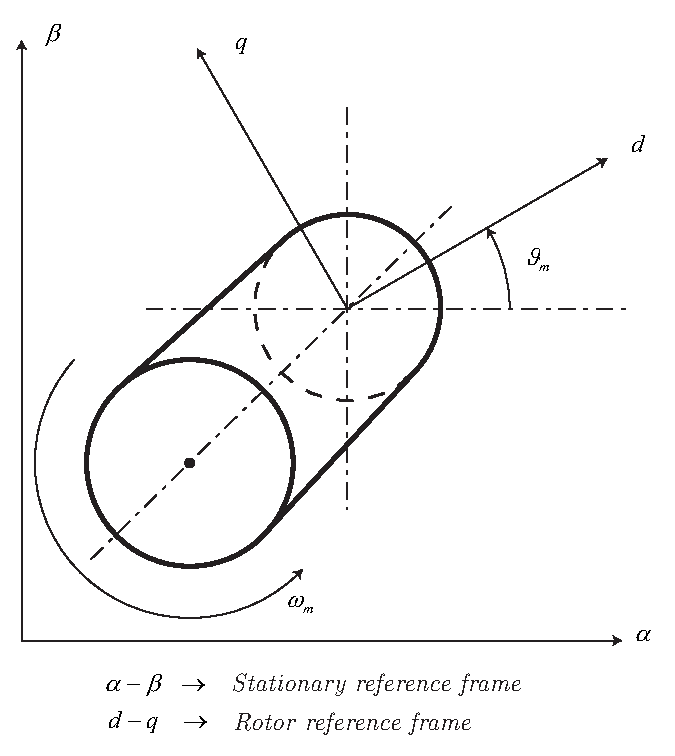
\includegraphics[width = 200pt, keepaspectratio]{figures/stationary_rotating_reference_frames.eps}
	\captionsetup{width=0.5\textwidth, font=small}		
	\caption{Stationary (stator) $(\alpha,\beta)$, rotor $(d,q)$.}
	\label{} 
\end{figure}
Hence
\begin{equation} \label{eq34}
	\left[
	\begin{matrix}
		i_{rd} \\[6pt]
		i_{rq}
	\end{matrix} \right] = 
	\left[
	\begin{matrix}
		\cos\vartheta_r & \sin\vartheta_r \\[6pt]
		-\sin\vartheta_r & \cos\vartheta_r \\[6pt]
	\end{matrix} \right]
	\left[
	\begin{matrix}
		i_{r\alpha} \\[6pt]
		i_{r\beta}
	\end{matrix} \right]
\end{equation}
\begin{equation} \label{eq35}
	\left[
	\begin{matrix}
		\psi_{rd} \\[6pt]
		\psi_{rq}
	\end{matrix} \right] = 
	\left[
	\begin{matrix}
		\cos\vartheta_r & \sin\vartheta_r \\[6pt]
		-\sin\vartheta_r & \cos\vartheta_r \\[6pt]
	\end{matrix} \right]
	\left[
	\begin{matrix}
		\psi_{r\alpha} \\[6pt]
		\psi_{r\beta}
	\end{matrix} \right]
\end{equation}
with $(\psi_{r\alpha},\psi_{r\beta})$ and $(i_{r\alpha}, i_{r\beta})$ denoting the $(\alpha,\beta)$-components of the rotor flux and current respect to a the fixed reference frame.
\begin{figure}[H]
	\centering
	\includegraphics[width = 400pt, keepaspectratio]{figures/reference_frames_2.eps}
	\captionsetup{width=0.5\textwidth, font=small}		
	\caption{Stationary (stator) $(\alpha,\beta)$, rotor (electrical) $(d,q)$ and synchronous speed $(x,y)$ reference frames.}
	\label{reference_frames} 
\end{figure}
Since
\begin{equation} \label{eq36}
	\begin{split}
		\left[
		\begin{matrix}
			\dot{\psi}_{r\alpha} \\[6pt]
			\dot{\psi}_{r\beta}
		\end{matrix} \right] = &
		\left[
		\begin{matrix}
			\cos\vartheta_r & -\sin\vartheta_r \\[6pt]
			\sin\vartheta_r & \cos\vartheta_r \\[6pt]
		\end{matrix} \right]
		\left[
		\begin{matrix}
			\dot{\psi}_{rd} \\[6pt]
			\dot{\psi}_{rq}
		\end{matrix} \right] + \omega_r
		\left[
		\begin{matrix}
			-\sin\vartheta_r & -\cos\vartheta_r \\[6pt]
			\cos\vartheta_r & -\sin\vartheta_r \\[6pt]
		\end{matrix} \right]
		\left[
		\begin{matrix}
			\psi_{rd} \\[6pt]
			\psi_{rq}
		\end{matrix} \right] \\[6pt]
		= & -
		\left[
		\begin{matrix}
			R_r & 0 \\[6pt]
			0 & R_r \\[6pt]
		\end{matrix} \right]
		\left[
		\begin{matrix}
			i_{r\alpha} \\[6pt]
			i_{r\beta}
		\end{matrix} \right] + 
		\left[
		\begin{matrix}
			-\omega_r{\psi}_{r\beta} \\[6pt]
			\omega_r{\psi}_{r\alpha}
		\end{matrix} \right]
	\end{split}
\end{equation}
we may write in $(i_{r\alpha}, i_{r\beta})$ coordinates
\begin{flalign} \label{eq37}
		\left[
		\begin{matrix}
			\dot{\psi}_{s\alpha} \\[6pt]
			\dot{\psi}_{s\beta}
		\end{matrix} \right] + 
		\left[
		\begin{matrix}
			R_s & 0 \\[6pt]
			0 & R_s \\[6pt]
		\end{matrix} \right]
		\left[
		\begin{matrix}
			i_{s\alpha} \\[6pt]
			i_{s\beta}
		\end{matrix} \right] = &
		\left[
		\begin{matrix}
			u_{s\alpha} \\[6pt]
			u_{s\beta}
		\end{matrix}
		\right] \\[6pt]
		\left[
		\begin{matrix}
			\dot{\psi}_{r\alpha} \\[6pt]
			\dot{\psi}_{r\beta}
		\end{matrix} \right] + 
		\left[
		\begin{matrix}
			R_r & 0 \\[6pt]
			0 & R_r \\[6pt]
		\end{matrix} \right]
		\left[
		\begin{matrix}
			i_{r\alpha} \\[6pt]
			i_{r\beta}
		\end{matrix} \right] + 
		\left[
		\begin{matrix}
			0 & \omega_r \\[6pt]
			- \omega_r & 0
		\end{matrix} \right]
		\left[
		\begin{matrix}
			{\psi}_{r\alpha} \\[6pt]
			{\psi}_{r\beta}
		\end{matrix} \right] = &
		\left[
		\begin{matrix}
			0 \\[6pt]
			0
		\end{matrix} \right]
\end{flalign}

The electromagnetic equations are
\begin{equation}\label{eq39}
	\left[\begin{matrix}
		\psi_{s\alpha} \\[6pt]
		\psi_{s\beta} \\[6pt]
		\psi_{r\alpha} \\[6pt]
		\psi_{r\beta} \\[6pt]
	\end{matrix}\right] = 
	\left[\begin{matrix}
		L_s & 0 & L_m & 0 \\[6pt]
		0 & L_s & 0 & L_m \\[6pt]
		L_m & 0 & L_r & 0 \\[6pt]
		0 & L_m & 0 & L_r \\[6pt]
	\end{matrix}\right]
	\left[\begin{matrix}
		i_{s\alpha} \\[6pt]
		i_{s\beta} \\[6pt]
		i_{r\alpha} \\[6pt]
		i_{r\beta} \\[6pt]
	\end{matrix}\right] = L
	\left[\begin{matrix}
		i_{s\alpha} \\[6pt]
		i_{s\beta} \\[6pt]
		i_{r\alpha} \\[6pt]
		i_{r\beta} \\[6pt]
	\end{matrix}\right]
\end{equation}
i.e. the quadratic form associated to $\mathbf{L}$
\begin{equation}\label{eq40}
	\frac{1}{2}\mathbf{i}^T\mathbf{L}\mathbf{i}
\end{equation}
is positive for any nonzero value of the current vector $\mathbf{i}=[i_{s\alpha}, i_{s\beta}, i_{r\alpha}, i_{r\beta}]$ and represent the magnetic energy.
Define 
\begin{equation}\label{eq42}
	\mathbf{R}=
	\left[\begin{matrix}
		R_s & 0 & 0 & 0 \\[6pt]
		0 & R_s & 0 & 0 \\[6pt]
		0 & 0 & R_r & 0 \\[6pt]
		0 & 0 & 0 & R_r \\[6pt]
	\end{matrix}\right]
\end{equation}
the first state space model is
\begin{flalign}
		\mathbf{L} &
		\left[\begin{matrix}
			\frac{d}{dt} i_{s\alpha} \\[6pt]
			\frac{d}{dt} i_{s\beta} \\[6pt]
			\frac{d}{dt} i_{r\alpha} \\[6pt]
			\frac{d}{dt} i_{r\beta}
		\end{matrix}\right] = -\mathbf{R}
		\left[\begin{matrix}
			i_{s\alpha} \\[6pt]
			i_{s\beta} \\[6pt]
			i_{r\alpha} \\[6pt]
			i_{r\beta} 
		\end{matrix}\right] + \\[6pt]
		+ &
		\left[\begin{matrix}
			0 & 0 & 0 & 0 \\[6pt]
			0 & 0 & 0 & 0 \\[6pt]
			0 & \omega_rL_m & 0 & \omega_rL_r \\[6pt]
			-\omega_rL_m & 0 & -\omega_rL_r & 0
		\end{matrix}\right]
		\left[\begin{matrix}
			i_{s\alpha} \\[6pt]
			i_{s\beta} \\[6pt]
			i_{r\alpha} \\[6pt]
			i_{r\beta} 
		\end{matrix}\right] + 
		\left[\begin{matrix}
			u_{s\alpha} \\[6pt]
			u_{s\beta} \\[6pt]
			0 \\[6pt]
			0
		\end{matrix}\right] \\[12pt]
		&
		\begin{matrix}
			J\frac{d}{dt}\omega_m = \tau_e-\tau_l
		\end{matrix}
\end{flalign}
in which the state variable are $(i_{s\alpha}, i_{s\beta}, i_{r\alpha}, i_{r\beta}, \omega_r)$ and the electromagnetic torque $\tau_e$ is still to be determined as a function of the state variables. This choice of state variables is naturally linked to the energy stored in the energy stored in the motor given by
\begin{equation}\label{eq43}
	E = \frac{1}{2}\mathbf{i}^T\mathbf{L}\mathbf{i}+\frac{1}{2}J\omega_m^2
\end{equation}
which is the sum of the magnetic energy and of the kinetic energy
\begin{equation}\label{eq44}
	\frac{1}{2}J\omega_m^2
\end{equation}
The expression of $\tau_e$ may be obtained from the energy balance
\begin{equation}\label{eq45}
	\begin{split}
		\frac{dE}{dt} = &
		\left[\begin{matrix}
			i_{s\alpha} i_{s\beta}
		\end{matrix}\right]
		\left[\begin{matrix}
			u_{s\alpha} u_{s\beta}
		\end{matrix}\right]^T -\tau_l\omega_m-\mathbf{i}^T\mathbf{R}\mathbf{i} + \\[6pt]
		& + \omega_m
		\left[\begin{matrix}
			i_{s\alpha} i_{s\beta}
		\end{matrix}\right]
		\left[\begin{matrix}
			0 & -L_m \\
			L_m & 0
		\end{matrix}\right]
		\left[\begin{matrix}
			i_{s\alpha} i_{s\beta}
		\end{matrix}\right]^T
		+\tau_e\omega_m
	\end{split}
\end{equation}
Let $P_{in}$, $P_{out}$ and $P_{loss}$ denote the input power, the output power, and the power losses, respectively; since
\begin{equation}\label{eq46}
	\begin{split}
		\frac{dE}{dt} = & P_{in} - P_{out} -P_{loss} \\[6pt]
		= &
		\left[\begin{matrix}
			i_{s\alpha} i_{s\beta}
		\end{matrix}\right]
		\left[\begin{matrix}
			u_{s\alpha} u_{s\beta}
		\end{matrix}\right]^T -\tau_l\omega_m-i^TRi
	\end{split}
\end{equation}
which means 
\begin{equation}\label{eq47}
	\tau_e = 
	\left[\begin{matrix}
		i_{s\alpha} i_{s\beta}
	\end{matrix}\right]
	\left[\begin{matrix}
		0 & -L_m \\
		L_m & 0
	\end{matrix}\right]
	\left[\begin{matrix}
		i_{s\alpha} i_{s\beta}
	\end{matrix}\right]^T = 
	L_m\left(i_{r\alpha} i_{s\beta} - i_{r\beta} i_{s\alpha}\right)
\end{equation}
Note that the electromagnetic torque $\tau_e$ produced by the motor is a nonlinear function of the state variables and constitutes the main nonlinear term in the induction motor model. Since
\begin{flalign}\label{eq48}
		i_{r\alpha} &= -\frac{L_m}{L_r}i_{s\alpha}+\frac{1}{Lr}\psi_{r\alpha} \\[6pt]
		i_{r\beta} &= -\frac{L_m}{L_r}i_{s\beta}+\frac{1}{Lr}\psi_{r\beta}
\end{flalign}
the electromagnetic torque may be expressed as
\begin{equation}\label{eq49}
	\tau_{e} = \frac{L_m}{L_r}\left(\psi_{r\alpha}i_{s\beta}-\psi_{r\beta}i_{s\alpha}\right).
\end{equation}
Eliminating $\left(\psi_{s\alpha}, \psi_{s\beta}, i_{r\alpha}, i_{r\beta}\right)$ from Eq.~\eqref{eq37} using equations \eqref{eq37} and \eqref{eq48}, namely
\begin{equation}\label{eq50}
	\left[\begin{matrix}
		i_{r\alpha} \\[6pt]
		i_{r\beta}
	\end{matrix}\right] = 
	\left[\begin{matrix}
		-\frac{L_m}{L_r} & 0 \\[6pt]
		0 & -\frac{L_m}{L_r}
	\end{matrix}\right]
	\left[\begin{matrix}
		i_{s\alpha} \\[6pt]
		i_{s\beta}
	\end{matrix}\right]+
	\left[\begin{matrix}
		\frac{1}{L_r} & 0 \\[6pt]
		0 & \frac{1}{L_r}
	\end{matrix}\right]
	\left[\begin{matrix}
		\psi_{r\alpha} \\[6pt]
		\psi_{r\beta}
	\end{matrix}\right]\\[6pt]
\end{equation}
\begin{equation}\label{eq51}
	\left[\begin{matrix}
		\psi_{s\alpha} \\[6pt]
		\psi_{s\beta}
	\end{matrix}\right] = 
	\left[\begin{matrix}
		L_s-\frac{L_m^2}{L_r} & 0 \\[6pt]
		0 & L_s-\frac{L_m^2}{L_r}
	\end{matrix}\right]
	\left[\begin{matrix}
		i_{s\alpha} \\[6pt]
		i_{s\beta}
	\end{matrix}\right]+
	\left[\begin{matrix}
		\frac{L_m}{L_r} & 0 \\[6pt]
		0 & \frac{L_m}{L_r}
	\end{matrix}\right]
	\left[\begin{matrix}
		\psi_{r\alpha} \\[6pt]
		\psi_{r\beta}
	\end{matrix}\right]
\end{equation}
we obtain a state model in terms of the state variables $\left(\omega_m, \psi_{r\alpha}, \psi_{r\beta},i_{s\alpha},i_{s\beta}\right)$ and the input variables $\left(u_{s\alpha}, u_{s\beta}, \tau_l\right)$

\begin{mybox}
	\textbf{The fixed frame model become}
	\begin{flalign}\label{eq52}
			\frac{d\omega_m}{dt} &= \mu \left(\psi_{r\alpha}i_{s\beta} - \psi_{r\beta}i_{s\alpha}\right)-\frac{\tau_l}{J} \\[6pt]
			\frac{d\psi_{r\alpha}}{dt} &= -\alpha \psi_{r\alpha} -\omega_r\psi_{r\beta}+\alpha L_m i_{s\alpha} \\[6pt]
			\frac{d\psi_{r\beta}}{dt} &= -\alpha \psi_{r\beta} +\omega_r\psi_{r\alpha}+\alpha L_m i_{s\beta} \\[6pt]
			\frac{di_{s\alpha}}{dt} &= -\gamma i_{s\alpha} + \frac{u_{s\alpha}}{\sigma} + \beta\alpha\psi_{r\alpha}+\beta\omega_r\psi_{r\beta} \\[6pt]
			\frac{di_{s\beta}}{dt} &= -\gamma i_{s\beta} + \frac{u_{s\beta}}{\sigma} + \beta\alpha\psi_{r\beta}-\beta\omega_r\psi_{r\alpha}
	\end{flalign}
	\textbf{where}
	\begin{flalign}\label{eq53}
			\mu & = \frac{L_m}{JL_r} \\[6pt]
			\alpha & = \frac{R_r}{L_r} \\[6pt]
			\sigma & = L_s \left(1-\frac{L_m^2}{L_sL_r}\right) \\[6pt]
			\beta & = \frac{L_m}{\sigma L_r} \\[6pt]
			\gamma & = \frac{R_s}{\sigma} + \beta \alpha L_m
	\end{flalign}
\end{mybox}
The state space model \eqref{eq52}, which will be referred to as fixed frame model, has some advantages from the control view point since it clarifies that the control inputs $\left(u_{s\alpha}\ u_{s\beta}\right)$ directly affect the dynamics of the stator currents $\left(i_{s\alpha}\ i_{s\beta}\right)$ which may be viewed as immediate control variables since they control the rotor speed $\omega_m$ and the rotor flux modulus $\sqrt{\psi_{r\alpha}^2 + \psi_{r\beta}^2}$ in the first three equations.

Let us now introduce a time-varying $\left(d,q\right)$ frame which rotates at an arbitrary speed $\omega_0(t)$ and is identified at each time $t$ by the angle $\vartheta_0(t)$ so that
\begin{equation}\label{eq54}
	\frac{d\vartheta_0}{dt} = \omega_0
\end{equation}
Rotor fluxes $(\psi_{r\alpha}, \psi_{r\beta})$, stator currents $(i_{s\alpha}, i_{s\beta})$, and stator voltages $(u_{s\alpha}, u_{s\beta})$ are expressed with respect to the time-varying rotating $(d,q)$ frame as 
\begin{flalign}\label{eq55}
		\left[
		\begin{matrix}
			\psi_{rd} \\[6pt]
			\psi_{rq}
		\end{matrix}
		\right] & =
		\left[
		\begin{matrix}
			\cos\vartheta_0 & \sin\vartheta_0 \\[6pt]
			-\sin\vartheta_0 & \cos\vartheta_0 \\[6pt]
		\end{matrix}
		\right]
		\left[
		\begin{matrix}
			\psi_{r\alpha} \\[6pt]
			\psi_{r\beta}
		\end{matrix}
		\right] \\[6pt]
		\left[
		\begin{matrix}
			i_{sd} \\[6pt]
			i_{sq}
		\end{matrix}
		\right] & =
		\left[
		\begin{matrix}
			\cos\vartheta_0 & \sin\vartheta_0 \\[6pt]
			-\sin\vartheta_0 & \cos\vartheta_0 \\[6pt]
		\end{matrix}
		\right]
		\left[
		\begin{matrix}
			i_{s\alpha} \\[6pt]
			i_{s\beta}
		\end{matrix}
		\right] \\[6pt]
		\left[
		\begin{matrix}
			u_{sd} \\[6pt]
			u_{sq}
		\end{matrix} 
		\right] & = 
		\left[
		\begin{matrix}
			\cos\vartheta_0 & \sin\vartheta_0 \\[6pt]
			-\sin\vartheta_0 & \cos\vartheta_0 \\[6pt]
		\end{matrix}
		\right]
		\left[
		\begin{matrix}
			u_{s\alpha} \\[6pt]
			u_{s\beta}
		\end{matrix}
		\right]
\end{flalign}
If the new \textbf{state variables} $(\omega_m, \psi_{rd}, \psi_{rq}, i_{sd}, i_{sq})$ and input variables $(u_{sd}, u_{sq}, \tau_l)$ are used, in the new $(d,q)$ rotating coordinates the induction motor model becomes
\begin{mybox}
	\textbf{The rotating frame model}
	\begin{flalign}\label{eq56}
			\frac{d\omega_m}{dt} &= \mu \left(\psi_{rd}i_{sq} - \psi_{rq}i_{sd}\right)-\frac{\tau_l}{J} \\[6pt]
			\frac{d\psi_{rd}}{dt} &= -\alpha \psi_{rd} +\left(\omega_0-\omega_r\right) \psi_{rq}+ \alpha L_m i_{sd} \\[6pt]
			\frac{d\psi_{rq}}{dt} &= -\alpha \psi_{rq}-\left(\omega_0-\omega_r\right) \psi_{rd}+\alpha L_m i_{sq} \\[6pt]
			\frac{di_{sd}}{dt} &= -\gamma i_{sd}  + \omega_0 i_{sq} + \beta\alpha\psi_{rd}+\beta\omega_r\psi_{rq} + \frac{u_{sd}}{\sigma} \\[6pt]
			\frac{di_{sq}}{dt} &= -\gamma i_{sq}  - \omega_0 i_{sd} + \beta\alpha\psi_{rq}-\beta\omega_r\psi_{rd} + \frac{u_{sq}}{\sigma}
	\end{flalign}
	where $\omega_0$ is the speed of the rotating reference frame
	\textbf{where}
	\begin{flalign}\label{eq57}
			\mu & = \frac{L_m}{JL_r} \\[6pt]
			\alpha & = \frac{R_r}{L_r} \\[6pt]
			\sigma & = L_s \left(1-\frac{L_m^2}{L_sL_r}\right) \\[6pt]
			\beta & = \frac{L_m}{\sigma L_r} \\[6pt]
			\gamma & = \frac{R_s}{\sigma} + \beta \alpha L_m
	\end{flalign}
\end{mybox}

In the case the rotating reference is attached to the rotor the induction motor model becomes
\begin{mybox}
	\textbf{The rotor frame model}
	\begin{flalign}\label{eq58}
		\frac{d\omega_m}{dt} &= \mu \left(\psi_{rd}i_{sq} - \psi_{rq}i_{sd}\right)-\frac{\tau_l}{J} \\[6pt]
		\frac{d\psi_{rd}}{dt} &= -\alpha \psi_{rd} + \alpha L_m i_{sd} \\[6pt]
		\frac{d\psi_{rq}}{dt} &= -\alpha \psi_{rq} + \alpha L_m i_{sq} \\[6pt]
		\frac{di_{sd}}{dt} &= -\gamma i_{sd}  + \omega_r i_{sq} + \beta\alpha\psi_{rd}+\beta\omega_r\psi_{rq} + \frac{u_{sd}}{\sigma} \\[6pt]
		\frac{di_{sq}}{dt} &= -\gamma i_{sq}  - \omega_r i_{sd} + \beta\alpha\psi_{rq}-\beta\omega_r\psi_{rd} + \frac{u_{sq}}{\sigma}
	\end{flalign}
	\textbf{The rotor frame state space model has some advantages from observability view point given by the linearity of the rotor flux equation where the cross terms are deleted from the selected rotating reference frame.}
\end{mybox}

\section{Rotor Flux Observer}
As mentioned in the previous chapter rotor flux may be observed by the implementation of the \textit{open-loop rotor flux observer}

\begin{mybox}
	\textbf{Open-loop rotor flux observer in the rotor frame model}
	\begin{flalign}\label{eq59}
		\frac{d\hat{\psi}_{rd}}{dt} &= -\alpha \hat{\psi}_{rd} + \alpha L_m i_{sd} \\[6pt]
		\frac{d\hat{\psi}_{rq}}{dt} &= -\alpha \hat{\psi}_{rq} + \alpha L_m i_{sq}
	\end{flalign}
	The flux observer errors $\hat{\psi}_{rd}(t) -{\psi}_{rd}(t)$ and $\hat{\psi}_{rq}(t) -{\psi}_{rq}(t)$ converge exponentially to zero with a rate of convergence $\alpha = \frac{R_r}{L_r}$. It requires the measurements of $\omega_m, i_{sd},i_{sq}$ and depends on the motor parameters $R_r$, $L_r$ and $L_m$. 
\end{mybox}
The same observer may be implemented in the fixed reference frame with the same properties.

\begin{mybox}
	\textbf{Open-loop rotor flux observer in the fixed frame model}
	\begin{flalign}\label{eq60}
			\frac{d\hat{\psi}_{r\alpha}}{dt} &= -\alpha \hat{\psi}_{r\alpha} -\omega_r\hat{\psi}_{r\beta} + \alpha L_m i_{s\alpha} \\[6pt]
			\frac{d\hat{\psi}_{r\beta}}{dt} &= -\alpha \hat{\psi}_{r\beta} +\omega_r\hat{\psi}_{r\alpha} + \alpha L_m i_{s\beta}
	\end{flalign}
	The flux observer errors $\hat{\psi}_{r\alpha}(t) -{\psi}_{r\alpha}(t)$ and $\hat{\psi}_{r\beta}(t) -{\psi}_{r\beta}(t)$ converge exponentially to zero with a rate of convergence $\alpha = \frac{R_r}{L_r}$. It requires the measurements of $\omega_m, i_{s\alpha},i_{s\beta}$ and depends on the motor parameters $R_r$, $L_r$ and $L_m$. 
\end{mybox}

The implementation of the \textbf{open-loop rotor flux observer in the rotor frame} becomes as follow
\begin{flalign}\label{eq61}
		\hat{\psi}_{rd}(k+1) &= \hat{\psi}_{rd}(k) + t_s\omega_{bez} \left[\alpha L_m i_{sd}(k) - \alpha\hat{\psi}(k)\right] \\[6pt]
		\hat{\psi}_{rq}(k+1) &= \hat{\psi}_{rq}(k) + t_s\omega_{bez} \left[\alpha L_m i_{sq}(k) - \alpha\hat{\psi}_{rq}(k)\right]
\end{flalign}
where $t_s$ is the sampling time of the digital representation and where the term $t_s\omega_{bez}$ derives from the normalization of the integration of a normalized quantity. 

The estimated slip phase is calculated by the function $\arctan2$ from the estimated rotor flux components $(\hat{\psi}_{rd}, \hat{\psi}_{rq})$
\begin{equation}\label{eq62}
	\hat{\vartheta}_{slip}=\atantwo(\hat{\psi}_{rd}, \hat{\psi}_{rq})
\end{equation}
the equivalent synchronous phase become 
\begin{equation}\label{eq63}
	\vartheta_{e}=\hat{\vartheta}_{slip}+\vartheta_{m}
\end{equation}
The correctness of the estimation of the slip phase $\hat{\vartheta}_{slip}$ affects the  behaviour of the machine; on the same time uncertainty of the parameter $R_r$ is the main cause of inaccuracy in the estimation of the rotor flux components, hence, of the slip phase. 


\section{Performance analysis and correction of the parameters}
In this section, the motor performance, under different condition of rotor resistance estimation, is investigated.

We denote with $R_r$ the real value of the rotor resistance whereas $R_r^p$ is the rotor resistance parameter applied to 
\begin{equation}\label{eq64}
	\alpha = \frac{R_r^p}{L_r^p}
\end{equation}
When rotor resistance parameter involved in the rotor flux estimation matches the real value of rotor resistance $R_r^p = R_r$, the estimated rotor flux $(\hat{\psi}_{rd}, \hat{\psi}_{rq})$ and the real $({\psi}_{rd}, {\psi}_{rq})$ are overlapped and the motor voltage at nominal speed is kept constant under different load condition. 

On the other side, when rotor parameter resistance doesn't match the real value of the rotor resistance and is under-estimated, that means $R_r^p < R_r$ the effects on the IM is equivalent to over-flux, in fact in this condition the real rotor-flux is proportionally increased, that means 
\begin{equation}\label{eq65}
	\left\{
	\begin{split} 
		R_r^p & = R_r  \Rightarrow \psi_r = \hat{\psi}_{r}  \\[6pt]
		R_r^p & < R_r  \Rightarrow \psi_r > \hat{\psi}_{r}  \Rightarrow \textrm{ \textit{over-flux condition}}
	\end{split}
	\right.
\end{equation}
As result, of the under estimation of the rotor resistance parameter, the machine is over-flux and the motor voltage, in load condition, is above the nominal value.

When rotor parameter resistance is over-estimated, that means $R_r^p > R_r$ the effects on the IM is equivalent to under-flux, in fact in this condition the real rotor-flux is proportionally decreased, that means 
\begin{equation}\label{eq66}
	\left\{
	\begin{split} 
		R_r^p & = R_r  \Rightarrow \psi_r = \hat{\psi}_{r}  \\[6pt]
		R_r^p & > R_r  \Rightarrow \psi_r < \hat{\psi}_{r}  \Rightarrow \textrm{ \textit{under-flux condition}}
	\end{split}
	\right.
\end{equation}
As result, of the over estimation of the rotor resistance parameter, the machine is under-flux and the motor voltage, in load condition, is below the nominal value.

\subsection{Motor performance under correct rotor resistance estimation}

\begin{figure}[H]
	\centering
	\begin{subfigure}{0.5\textwidth}
	\centering
	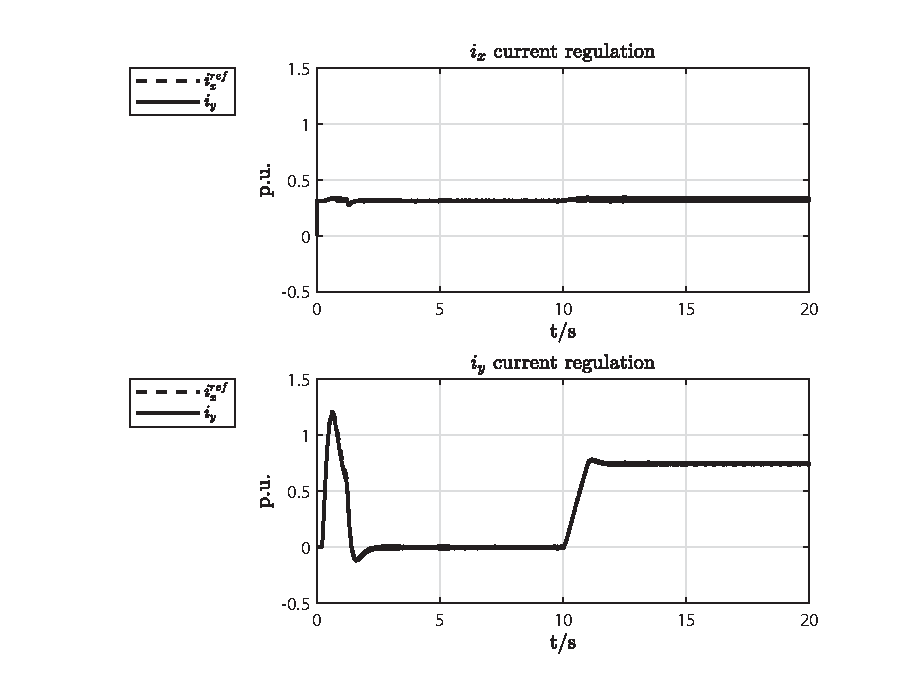
\includegraphics[width = 240pt, keepaspectratio]{figures/equal/current_reg.eps}
	\captionsetup{width=0.65\textwidth, font=footnotesize}	
	\caption{Stator current regulation in $(x,y)$ coordinates - synchronous reference frame.}
	\label{fig_sim_res_1}
	\end{subfigure}%
	\begin{subfigure}{0.5\textwidth}
	\centering
	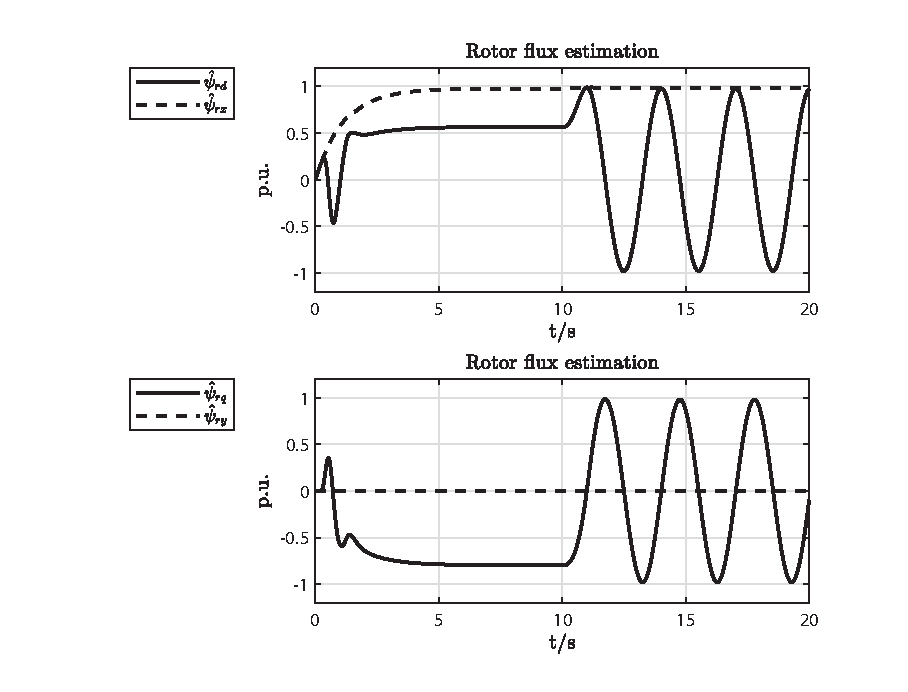
\includegraphics[width = 240pt, keepaspectratio]{figures/equal/rotor_flux_est_1.eps}
	\captionsetup{width=0.65\textwidth, font=footnotesize}	
	\caption{Estimated rotor flux $(d,q)$-(rotor frame) and $(x,y)$-(synchronous frame) coordinates.}
	\label{fig_sim_res_2}
	\end{subfigure}		
	\captionsetup{width=0.5\textwidth, font=small}		
	\caption{Motor performance under correct rotor resistance estimation.}
	\label{}
\end{figure}

\begin{figure}[H]
	\centering
	\begin{subfigure}{0.5\textwidth}
	\centering
	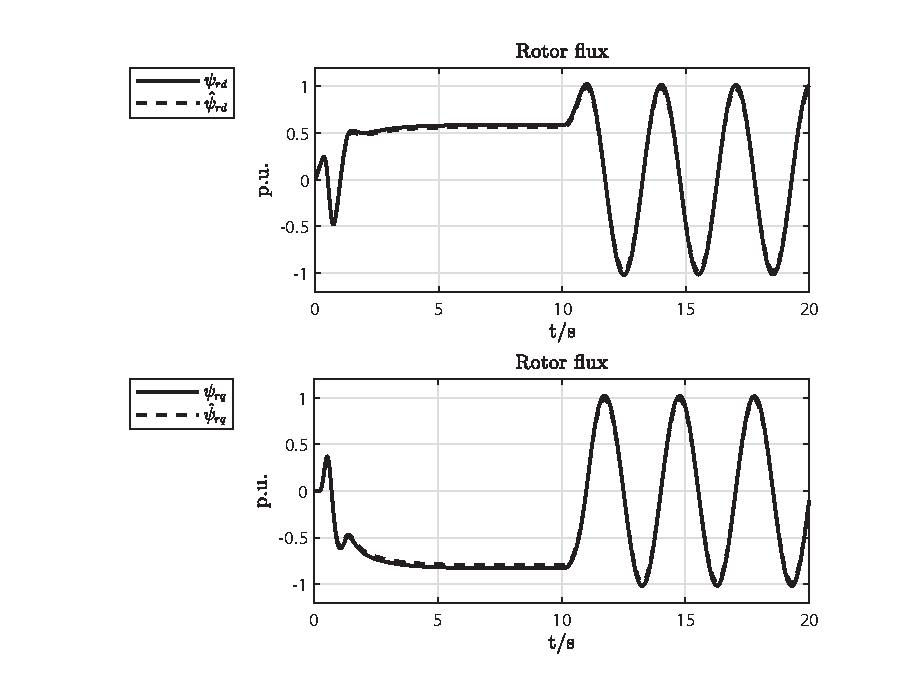
\includegraphics[width = 240pt, keepaspectratio]{figures/equal/rotor_flux_est_2.eps}
	\captionsetup{width=0.65\textwidth, font=footnotesize}	
	\caption{Estimated (dashed) and real (solid) rotor flux in $(d,q)$-(rotor frame) coordinates.}
	\label{fig_sim_res_3}
	\end{subfigure}%
	\begin{subfigure}{0.5\textwidth}
	\centering
	\includegraphics[width = 240pt, keepaspectratio]{figures/equal/motor_voltage.eps}
	\captionsetup{width=0.65\textwidth, font=footnotesize}	
	\caption{Motor voltage (phase to phase rms) and torques (electromagnetic and load).}
	\label{fig_sim_res_4}
	\end{subfigure}		
	\captionsetup{width=0.5\textwidth, font=small}	
	\caption{Motor performance under correct rotor resistance estimation.}
	\label{}
\end{figure}

\subsection{Motor performance with underestimate rotor resistance}

\begin{figure}[H]
	\centering
	\begin{subfigure}{0.5\textwidth}
	\centering
	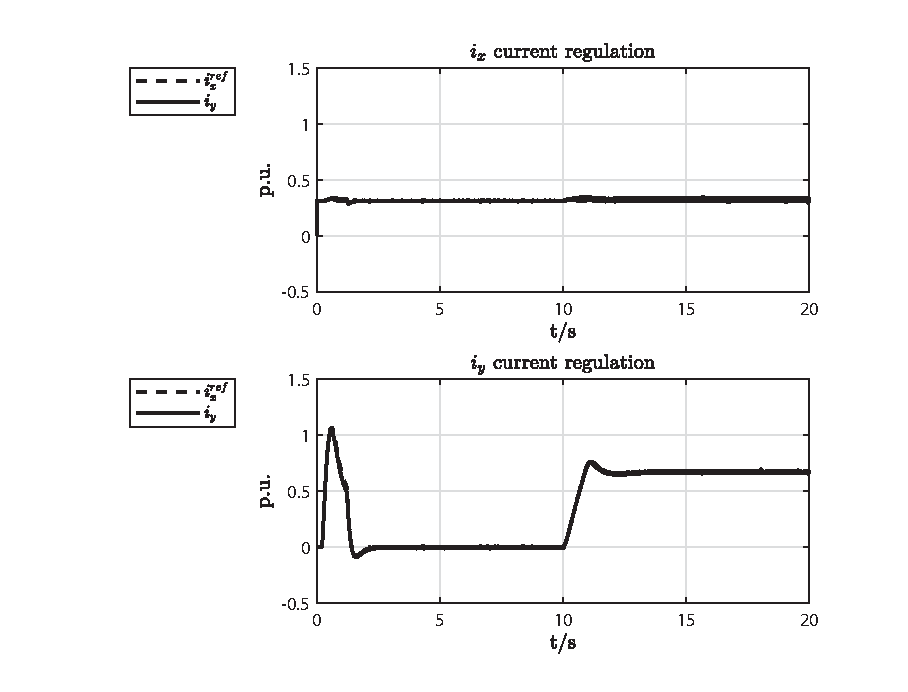
\includegraphics[width = 240pt, keepaspectratio]{figures/under_est/current_reg.eps}
	\captionsetup{width=0.65\textwidth, font=footnotesize}		
	\caption{Stator current regulation in $(x,y)$ coordinates - synchronous reference frame - \textit{under-estimation case}.}
	\label{fig_sim_res_5}
	\end{subfigure}%
	\begin{subfigure}{0.5\textwidth}
	\centering
	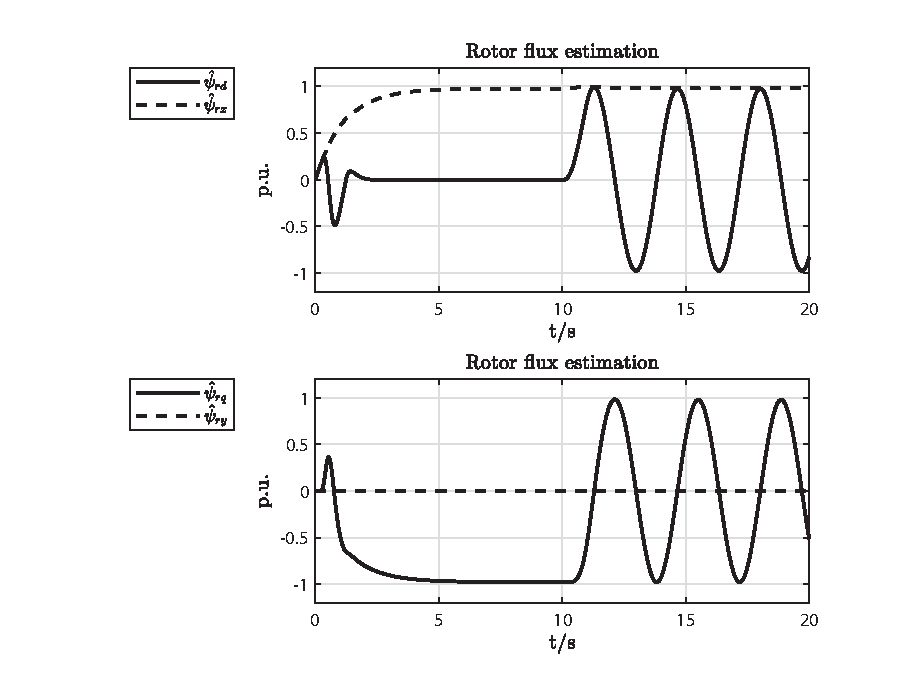
\includegraphics[width = 240pt, keepaspectratio]{figures/under_est/rotor_flux_est_1.eps}
	\captionsetup{width=0.65\textwidth, font=footnotesize}		
	\caption{Estimated rotor flux $(d,q)$-(rotor frame) and $(x,y)$-(synchronous frame) coordinates - \textit{under-estimation case}.}
	\label{fig_sim_res_6}
	\end{subfigure}		
	\captionsetup{width=0.5\textwidth, font=small}		
	\caption{Motor performance with underestimate rotor resistance.}
	\label{}
\end{figure}

\begin{figure}[H]
	\centering
	\begin{subfigure}{0.5\textwidth}
	\centering
	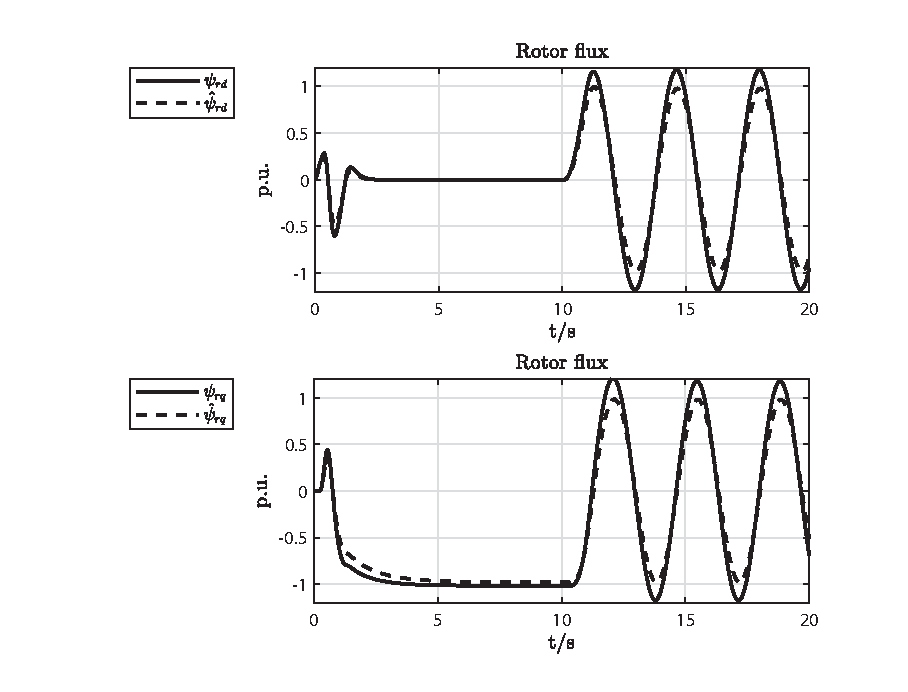
\includegraphics[width = 240pt, keepaspectratio]{figures/under_est/rotor_flux_est_2.eps}
	\captionsetup{width=0.65\textwidth,font=footnotesize}		
	\caption{Estimated (dashed) and real (solid) rotor flux in $(d,q)$-(rotor frame) coordinates - \textit{under-estimation case}.}
	\label{fig_sim_res_7}
	\end{subfigure}%
	\begin{subfigure}{0.5\textwidth}
	\centering
	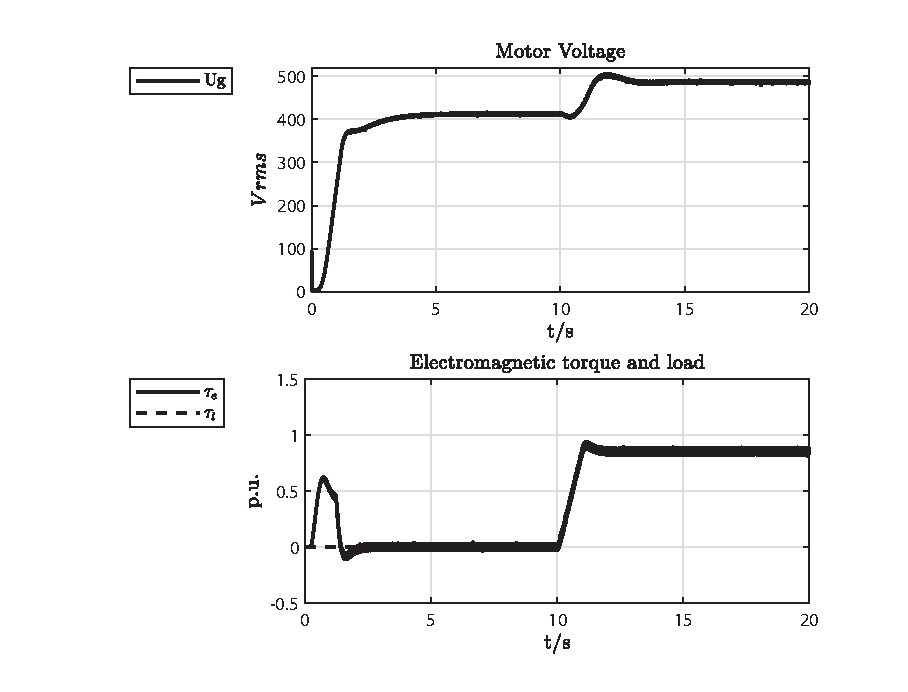
\includegraphics[width = 240pt, keepaspectratio]{figures/under_est/motor_voltage.eps}
	\captionsetup{width=0.65\textwidth,font=footnotesize}		
	\caption{Motor voltage (phase to phase rms) and torques (electromagnetic and load) - \textit{under-estimation case}.}
	\label{fig_sim_res_8}
	\end{subfigure}		
	\captionsetup{width=0.5\textwidth, font=small}		
	\caption{Motor performance with underestimate rotor resistance.}
	\label{}
\end{figure}

\subsection{Motor performance with overestimate rotor resistance}

\begin{figure}[H]
	\centering
	\begin{subfigure}{0.5\textwidth}
	\centering
	\includegraphics[width = 240pt, keepaspectratio]{figures/over_est/current_reg.eps}
	\captionsetup{width=0.65\textwidth, font=footnotesize}		
	\caption{Stator current regulation in $(x,y)$ coordinates - synchronous reference frame - \textit{over-estimation case}.}
	\label{fig_sim_res_9}
	\end{subfigure}%
	\begin{subfigure}{0.5\textwidth}
	\centering
	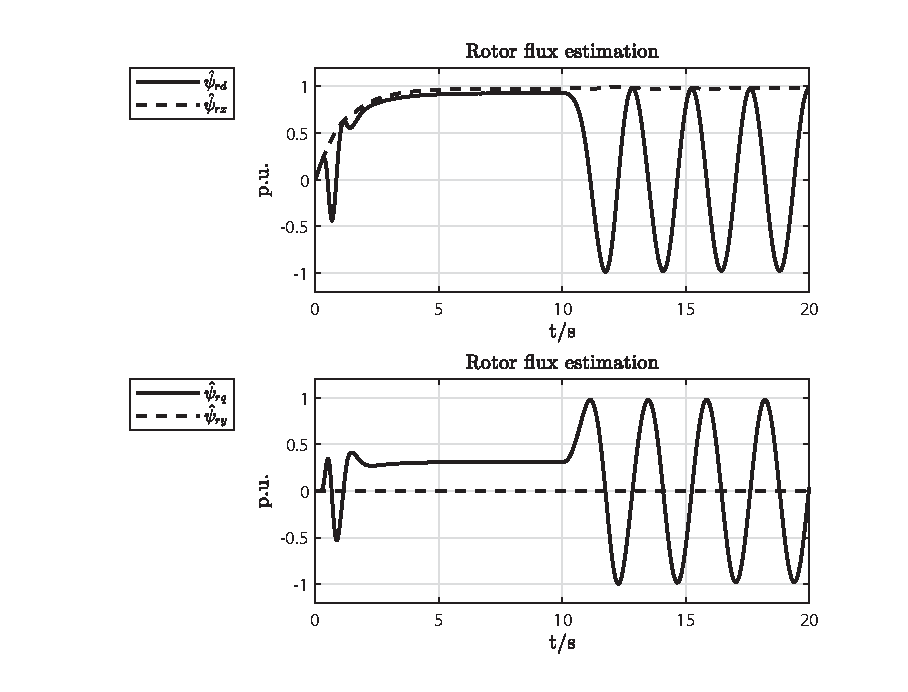
\includegraphics[width = 240pt, keepaspectratio]{figures/over_est/rotor_flux_est_1.eps}
	\captionsetup{width=0.65\textwidth, font=footnotesize}		
	\caption{Estimated rotor flux $(d,q)$-(rotor frame) and $(x,y)$-(synchronous frame) coordinates - \textit{over-estimation case}.}
	\label{fig_sim_res_10}
	\end{subfigure}		
	\captionsetup{width=0.5\textwidth, font=small}		
	\caption{Motor performance with overestimate rotor resistance.}
	\label{}
\end{figure}

\begin{figure}[H]
	\centering
	\begin{subfigure}{0.5\textwidth}
	\centering
	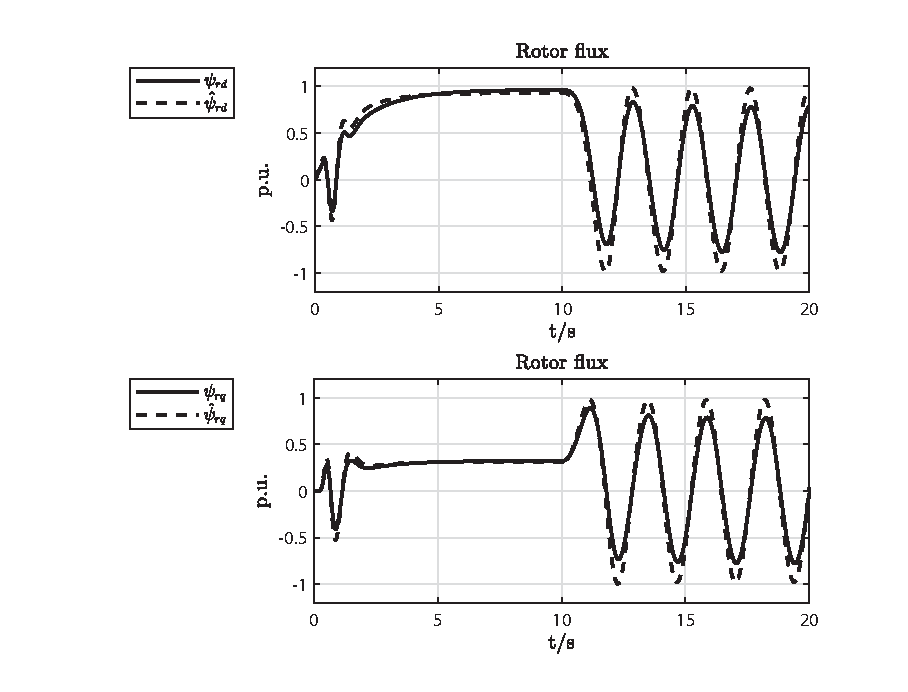
\includegraphics[width = 240pt, keepaspectratio]{figures/over_est/rotor_flux_est_2.eps}
	\captionsetup{width=0.65\textwidth, font=footnotesize}	
	\caption{Estimated (dashed) and real (solid) rotor flux in $(d,q)$-(rotor frame) coordinates - \textit{over-estimation case}.}
	\label{fig_sim_res_11}
	\end{subfigure}%
	\begin{subfigure}{0.5\textwidth}
	\centering
	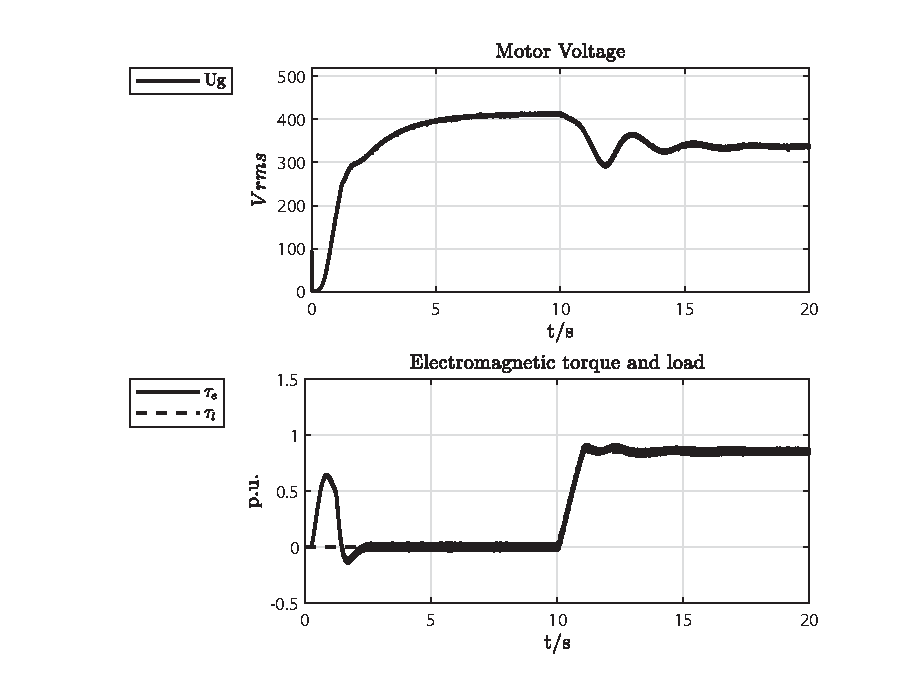
\includegraphics[width = 240pt, keepaspectratio]{figures/over_est/motor_voltage.eps}
	\captionsetup{width=0.65\textwidth, font=footnotesize}	
	\caption{Motor voltage (phase to phase rms) and torques (electromagnetic and load) - \textit{over-estimation case}.}
	\label{fig_sim_res_12}
	\end{subfigure}		
	\captionsetup{width=0.5\textwidth, font=small}		
	\caption{Motor performance with overestimate rotor resistance.}
	\label{}
\end{figure}

\chapter{Online Rotor Resistance Estimation}
\section{Introduction}
In this chapter we summarize the comparison between different rotor resistance estimator algorithms which have been implemented and tested.

Before to start with the description of the algorithms we just introduce some clarification between different type of observers. 

It is commonly to distinguish between two kind of observers:
\begin{myitemize_3}
	\item[--] \textit{a priori} observer also called \text{without constraint} or open-loop;
	\item[--] \textit{a posteriori} observer also called \text{with constraint} or closed-loop.
\end{myitemize_3}

The \textit{a priori} observer results of the form
\begin{equation}
	\begin{split}
		\dot{\hat{\boldsymbol{x}}} & = \boldsymbol{A} \hat{\boldsymbol{x}} + \boldsymbol{B}\boldsymbol{u} \\[6pt]
		\hat{\boldsymbol{y}} & = \boldsymbol{C}\hat{\boldsymbol{x}}
	\end{split}
\end{equation}
The \textit{a posteriori} observer results of the form
\begin{equation}
	\begin{split}
		\dot{\hat{\boldsymbol{x}}} & = \boldsymbol{A} \hat{\boldsymbol{x}} + \boldsymbol{B}\boldsymbol{u}
		 + \boldsymbol{L}\left(\boldsymbol{y}-\hat{\boldsymbol{y}}\right)\\[6pt]
		\hat{\boldsymbol{y}} & = \boldsymbol{C}\hat{\boldsymbol{x}}
	\end{split}
\end{equation}
where $\boldsymbol{y}$ is a measured output quantity.

Remains the fact that in both observers part of the $\hat{\boldsymbol{x}}$ state is measured.

Moving to induction motor and on rotor resistance estimators, the following algorithms were been implemented
\begin{itemize}
	\item A. Ba-Razzouk, A. Cheriti \textit{Implementation of DSP Based Real-Time Estimator of Induction Motor Rotor Time Constant}. IEEE Transaction on Power Electronics 2000.
	\item R. Marino, P. Tomei C. M. Verrelli \textit{Adaptive flux observer with rotor resistance estimator} - Chp. 3 - Induction Motor Control Design. Springer 2010.
	\item G. Kenne, R. S. Simo, F. Lamnabhi-Lagarrigue, A. Arzande, J.C. Vannier. \textit{An Online Simplified Rotor Resistance Estimator for Induction Motor} - IEEE Transaction on Power Electronics 2010.
\end{itemize}

In the first publication, basically, the rotor resistance estimation is performed by a simple open-loop observer. Experimental results show a not robust algorithm and the global performance poor and strongly sensitive to the accuracy of the input voltage $u = \left(u_{s\alpha}, u_{s\beta}\right)$ applied to the observer and to the motor.

The rest of publications are both based on the fundamental work of \textbf{Marino-Peresada} \textit{On-Line Stator and Rotor Resistance Estimation for Induction Motors} IEEE Transaction on Control Systems Technology 2000, where fluxes and rotor resistance estimation are based on a closed loop observers where the \textit{a posteriori} constraint is the error of the closed loop estimation of the stator currents $\tilde{i}_{s\alpha} = i_{s\alpha} - \hat{i}_{s\alpha}$ and $\tilde{i}_{s\beta} = i_{s\beta} - \hat{i}_{s\beta}$.

The algorithm of Marino-Tomei-Verrelli was only partially implemented, in fact the flux estimation from this algorithm (closed loop form) were not used in the main control loop in order to keep the original flux estimation (open loop form). The reason of that was to avoid changing in the original control structure. The missing closed loop flux observer in the main control could be a strong cause of the not robust performance, and the estimation of the rotor resistance was strongly dependent by the load and by the selected gains.

The last control algorithm, proposed in the above list, as been tested with good results in term of performance and robustness. 

In the following, both algorithms \textit{Adaptive flux observer with rotor resistance estimator}, and \textit{An Online Simplified Rotor Resistance Estimator for Induction Motor} will be presented.

\newpage
\begin{mybox}
	\textbf{Adaptive flux observer with rotor resistance estimator} - The controller is performed in the stationary reference frame.

	\begin{flalign}\label{eq67}
			\tilde{i}_{s\alpha} &= i_{s\alpha} - \hat{i}_{s\alpha} \\[6pt]
			\tilde{i}_{s\beta} &= i_{s\beta} - \hat{i}_{s\beta} \\[6pt]
			\frac{d\hat{i}_{s\alpha}}{dt} &= -\frac{R_s}{\sigma}\hat{i}_{s\alpha} - \hat{\alpha} \left(1+\beta L_m\right) i_{s\alpha} + \omega_r \hat{i}_{s\beta} + \hat{\alpha}\hat{\eta}_{\alpha} + \omega_r \hat{z}_{\beta} + \frac{1}{\sigma} u_{s\alpha} + k_1 \tilde{i}_{s\alpha} \\[6pt]
			\frac{d\hat{i}_{s\beta}}{dt} &= -\frac{R_s}{\sigma}\hat{i}_{s\beta} - \hat{\alpha} \left(1+\beta L_m\right) i_{s\beta} + \omega_r \hat{i}_{s\alpha} + \hat{\alpha}\hat{\eta}_{\beta} + \omega_r \hat{z}_{\alpha} + \frac{1}{\sigma} u_{s\beta} + k_1 \tilde{i}_{s\beta} \\[6pt]
			\frac{d\hat{z}_{\alpha}}{dt} &= -\frac{R_s}{\sigma} i_{s\alpha} + \frac{1}{\sigma} u_{s\alpha} - k_2 \omega_r \tilde{i}_{s\beta} \\[6pt]
			\frac{d\hat{z}_{\beta}}{dt} &= -\frac{R_s}{\sigma} i_{s\beta} + \frac{1}{\sigma} u_{s\beta} + k_2 \omega_r \tilde{i}_{s\alpha} \\[6pt]
			\frac{d\hat{\eta}_{\alpha}}{dt} &= -\frac{R_s}{\sigma} i_{s\alpha} + \frac{1}{\sigma} u_{s\alpha} + k_3 \tilde{i}_{s\alpha} \\[6pt]
			\frac{d\hat{\eta}_{\beta}}{dt} &= -\frac{R_s}{\sigma} i_{s\beta} + \frac{1}{\sigma} u_{s\beta} + k_3 \tilde{i}_{s\beta} \\[6pt]
			\frac{d\hat{\alpha}}{dt} &= - g\left\{\left[\left(1+\beta L_m\right)i_{s\alpha}-\hat{\eta}_{\alpha}\right]\tilde{i}_{s\alpha} + \left[\left(1+\beta L_m \right)i_{s\beta}-\hat{\eta}_{\beta}\right]\tilde{i}_{s\beta} \right\}
	\end{flalign}
	\begin{flalign}\label{eq68}
			\mu & = \frac{L_m}{JL_r} \\[6pt]
			\alpha & = \frac{R_r}{L_r} \\[6pt]
			\sigma & = L_s \left(1-\frac{L_m^2}{L_sL_r}\right) \\[6pt]
			\beta & = \frac{L_m}{\sigma L_r} \\[6pt]
			\gamma & = \frac{R_s}{\sigma} + \beta \alpha L_m
	\end{flalign}
\end{mybox}

\newpage
\begin{mybox}
	\textbf{Simplified rotor resistance estimator} - The controller is performed in the stationary reference frame.
	
	\noindent Starting from the flux and current equation 
	\begin{flalign}\label{eq69}
			\frac{di_{s\alpha}}{dt} &= -\frac{R_s}{\sigma L_s}{i}_{s\alpha} - \beta L_m \frac{{R_r}}{L_r} i_{s\alpha} +\beta \frac{{R_r}}{L_r} {\psi}_{r\alpha} + \omega_r \beta {\psi}_{r\beta} +\frac{1}{\sigma L_s} u_{s\alpha} \\[6pt]
			\frac{di_{s\beta}}{dt} &= -\frac{R_s}{\sigma L_s}{i}_{s\beta} - \beta L_m \frac{{R_r}}{L_r} i_{s\beta} +\beta \frac{{R_r}}{L_r} {\psi}_{r\beta} - \omega_r \beta {\psi}_{r\alpha} +\frac{1}{\sigma L_s} u_{s\beta} \\[6pt]
			\frac{d{\psi}_{r\alpha}}{dt} &= -\frac{{R_r}}{L_r}{\psi}_{r\alpha} - \omega_r {\psi}_{r\beta} +\frac{{R_r}}{L_r} L_m {i}_{s\alpha} \\[6pt]
			\frac{d{\psi}_{r\beta}}{dt} &= -\frac{{R_r}}{L_r}{\psi}_{r\beta} + \omega_m {\psi}_{r\alpha} +\frac{{R_r}}{L_r} L_m {i}_{s\beta}
	\end{flalign}
	\begin{flalign}\label{eq70}
			\sigma & = \left(1-\frac{L_m^2}{L_sL_r}\right) \\[6pt]
			\beta & = \frac{L_m}{\sigma L_r L_s} 
	\end{flalign}%
	The full observers equations are%
	\begin{flalign}\label{eq71}
			\tilde{i}_{s\alpha} &= i_{s\alpha} - \hat{i}_{s\alpha} \\[6pt]
			\tilde{i}_{s\beta} &= i_{s\beta} - \hat{i}_{s\beta} \\[6pt]
			\frac{d\hat{i}_{s\alpha}}{dt} &= -\frac{R_s}{\sigma L_s}{i}_{s\alpha} - \beta L_m \frac{\hat{R_r}}{L_r} i_{s\alpha} +\beta \frac{\hat{R_r}}{L_r} \hat{\psi}_{r\alpha} + \omega_r \beta \hat{\psi}_{r\beta} \\[6pt]
			&+\frac{1}{\sigma L_s} u_{s\alpha} + k_1 \sign\left(\tilde{i}_{s\alpha}\right) \\[6pt]
			\frac{d\hat{i}_{s\beta}}{dt} &= -\frac{R_s}{\sigma L_s}{i}_{s\beta} - \beta L_m \frac{\hat{R_r}}{L_r} i_{s\beta} +\beta \frac{\hat{R_r}}{L_r} \hat{\psi}_{r\beta} - \omega_r \beta \hat{\psi}_{r\alpha} \\[6pt]
			&+\frac{1}{\sigma L_s} u_{s\beta} + k_1 \sign\left(\tilde{i}_{s\beta}\right) \\[6pt]
			\frac{d\hat{\psi}_{r\alpha}}{dt} &= -\frac{\hat{R_r}}{L_r}\hat{\psi}_{r\alpha} - \omega_r \hat{\psi}_{r\beta} +\frac{\hat{R_r}}{L_r} L_m {i}_{s\alpha} +\xi_{\alpha} \\[6pt]
			\frac{d\hat{\psi}_{r\beta}}{dt} &= -\frac{\hat{R_r}}{L_r}\hat{\psi}_{r\beta} + \omega_r \hat{\psi}_{r\alpha} +\frac{\hat{R_r}}{L_r} L_m {i}_{s\beta} +\xi_{\beta}
	\end{flalign}
	\begin{flalign}\label{eq72}		
		\xi_{\alpha} &= \frac{\tilde{R_r}}{L_r} \left(L_m i_{s\alpha} - \hat{\psi}_{r\alpha}\right) \\[6pt]
		\xi_{\beta} &= \frac{\tilde{R_r}}{L_r} \left(L_m i_{s\beta} - \hat{\psi}_{r\beta}\right) \\[6pt]
		\dot{\hat{R_r}} &= k_r \sign \left(\tilde{R_r}\right) \\[6pt]
		\tilde{R_r} &= \frac{L_r}{\beta} \frac{\left[\hat{\psi}_r - L_m i_s\right]^T W_{eq}}{\| \hat{\psi}_r - L_m i_s \|^2} \\[6pt]
		W_{eq}^T &= \left(W_{\alpha eq}, W_{\beta eq}\right) \\[6pt]
		W_{\alpha eq} &= k_1 \sign \left(\tilde{i}_{s\alpha}\right) \Rightarrow \text{This quantity shall be filtered} \\[6pt]
		W_{\beta eq} &= k_1 \sign \left(\tilde{i}_{s\beta}\right) \Rightarrow \text{This quantity shall be filtered}
	\end{flalign}
\end{mybox}

\section{Simulation results of the simplified rotor resistance estimator}

\subsection{Induction motor in hot condition}
\begin{figure}[H]
	\centering
	\begin{subfigure}{0.5\textwidth}
	\centering
	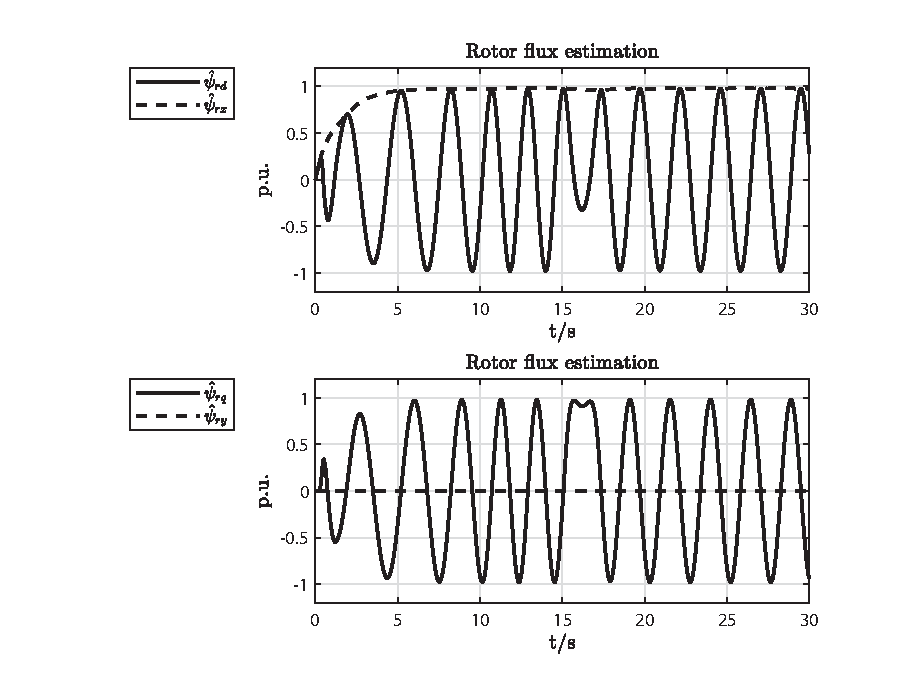
\includegraphics[width = 240pt, keepaspectratio]{figures/sim_results/hot_condition/rotor_flux_est_1.eps}
	\captionsetup{width=0.65\textwidth, font=footnotesize}	
	\caption{Estimated rotor flux $(d,q)$-(rotor frame) and $(x,y)$-(synchronous frame) coordinates - $R_r^p < R_r$.}
	\label{fig_sim_res_13}
	\end{subfigure}%
	\begin{subfigure}{0.5\textwidth}
	\centering
	\includegraphics[width = 240pt, keepaspectratio]{figures/sim_results/hot_condition/rotor_flux_est_2.eps}
	\captionsetup{width=0.65\textwidth, font=footnotesize}	
	\caption{Estimated (dashed) and real (solid) rotor flux in $(d,q)$-(rotor frame) coordinates - $R_r^p < R_r$.}
	\label{fig_sim_res_14}
	\end{subfigure}		
	\captionsetup{width=0.5\textwidth, font=small}		
	\caption{Induction motor in hot condition.}
	\label{}
\end{figure}

\begin{figure}[H]
	\centering
	\begin{subfigure}{0.5\textwidth}
	\centering
	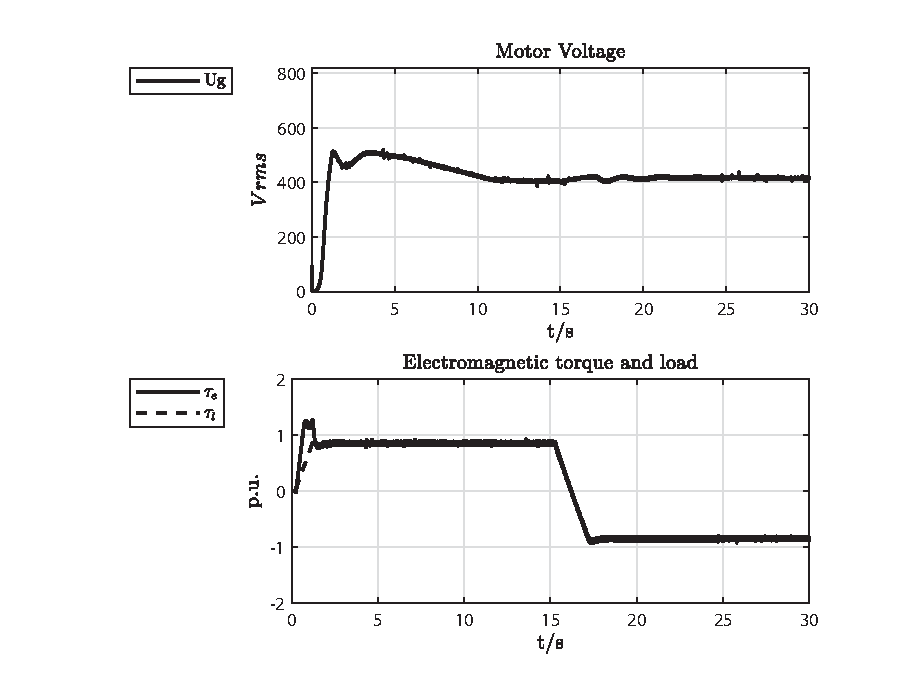
\includegraphics[width = 240pt, keepaspectratio]{figures/sim_results/hot_condition/motor_voltage.eps}
	\captionsetup{width=0.65\textwidth, font=footnotesize}	
	\caption{Motor voltage (phase to phase rms) and torques (electromagnetic and load) - $R_r^p < R_r$.}
	\label{fig_sim_res_15}
	\end{subfigure}%
	\begin{subfigure}{0.5\textwidth}
	\centering
	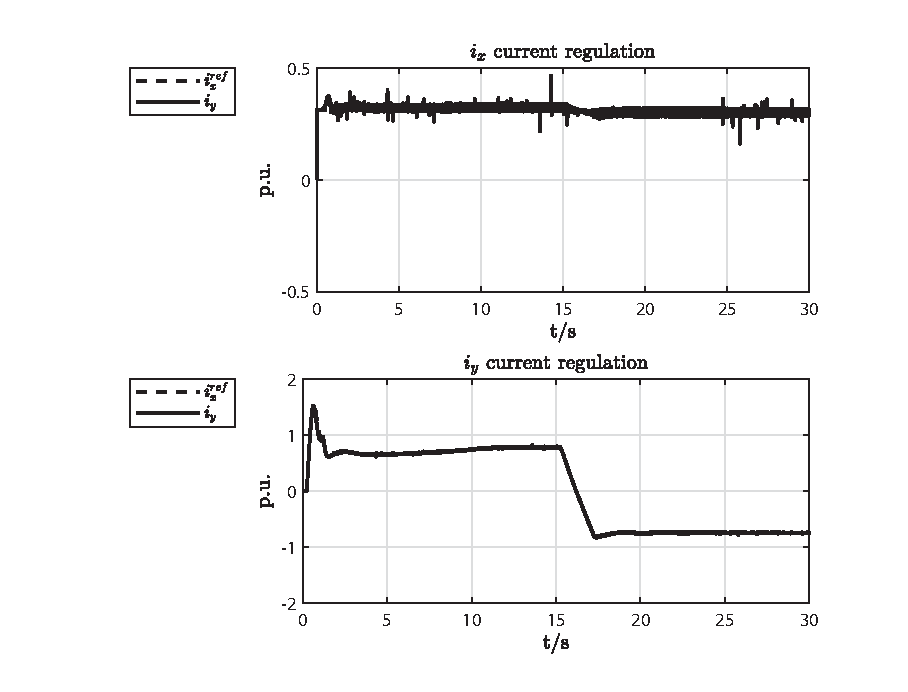
\includegraphics[width = 240pt, keepaspectratio]{figures/sim_results/hot_condition/current_reg.eps}
	\captionsetup{width=0.65\textwidth, font=footnotesize}	
	\caption{Stator current regulation in $(x,y)$ coordinates - synchronous reference frame - $R_r^p < R_r$.}
	\label{fig_sim_res_16}
	\end{subfigure}		
	\captionsetup{width=0.5\textwidth, font=small}		
	\caption{Induction motor in hot condition.}
	\label{}
\end{figure}

\begin{figure}[H]
	\centering
	\begin{subfigure}{0.5\textwidth}
	\centering
	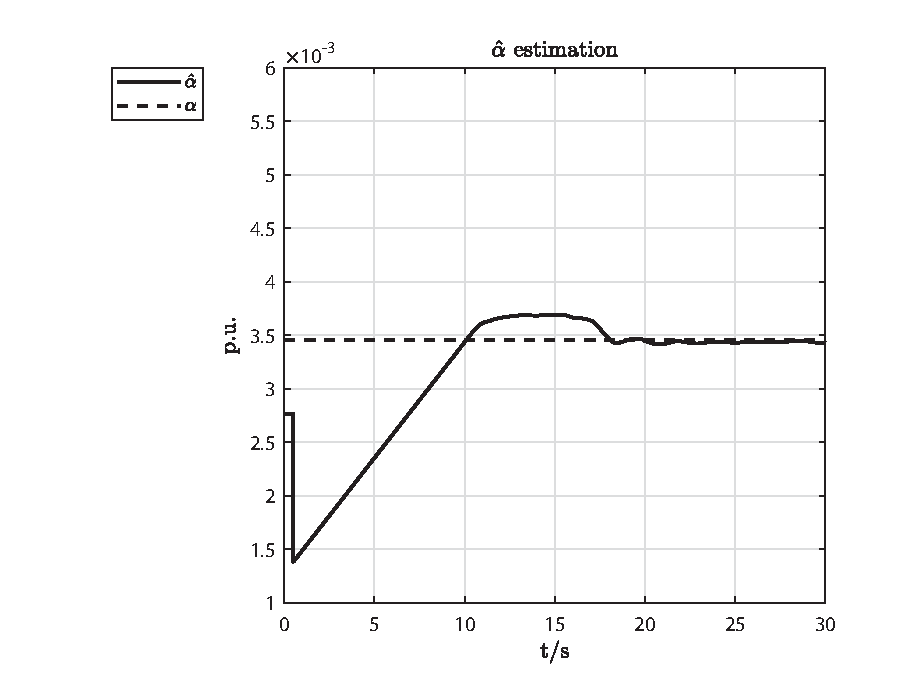
\includegraphics[width = 240pt, keepaspectratio]{figures/sim_results/hot_condition/alpha_est.eps}
	\captionsetup{width=0.65\textwidth, font=footnotesize}	
	\caption{Rotor ${\alpha}$ estimation - $R_r^p < R_r$.}
	\label{fig_sim_res_17}
	\end{subfigure}%
	\begin{subfigure}{0.5\textwidth}
	\centering
	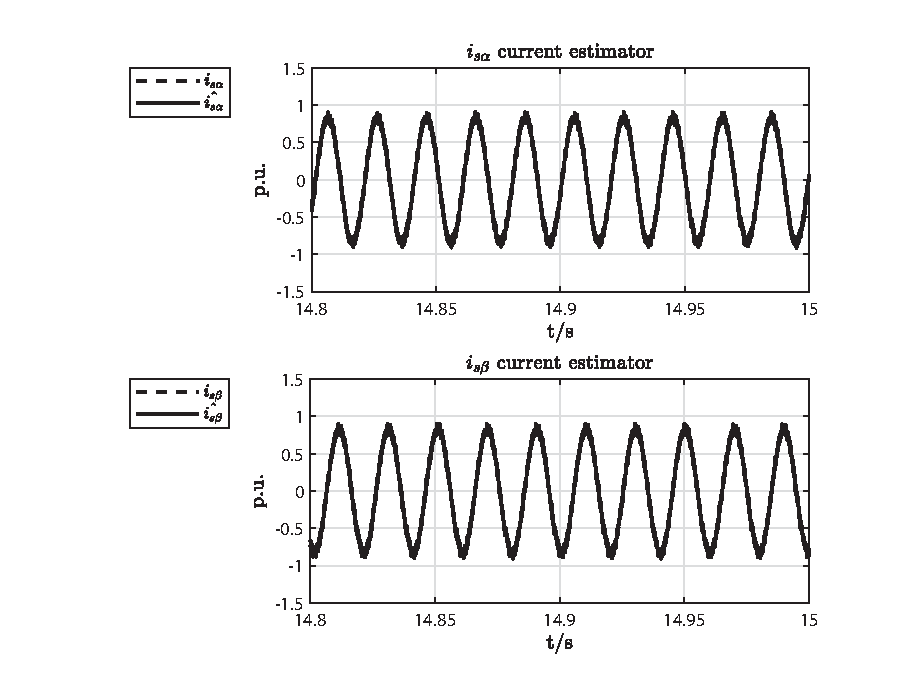
\includegraphics[width = 240pt, keepaspectratio]{figures/sim_results/hot_condition/current_obs.eps}
	\captionsetup{width=0.65\textwidth, font=footnotesize}	
	\caption{Stator current observer - $R_r^p < R_r$.}
	\label{fig_sim_res_18}
	\end{subfigure}		
	\captionsetup{width=0.5\textwidth, font=small}		
	\caption{Induction motor in hot condition.}
	\label{}
\end{figure}

\subsection{Induction motor in cold condition}

\begin{figure}[H]
	\centering
	\begin{subfigure}{0.5\textwidth}
	\centering
	\includegraphics[width = 240pt, keepaspectratio]{figures/sim_results/cold_condition/rotor_flux_est_1.eps}
	\captionsetup{width=0.65\textwidth, font=footnotesize}	
	\caption{Estimated rotor flux $(d,q)$-(rotor frame) and $(x,y)$-(synchronous frame) coordinates - $R_r^p > R_r$.}
	\label{fig_sim_res_19}
	\end{subfigure}%
	\begin{subfigure}{0.5\textwidth}
	\centering
	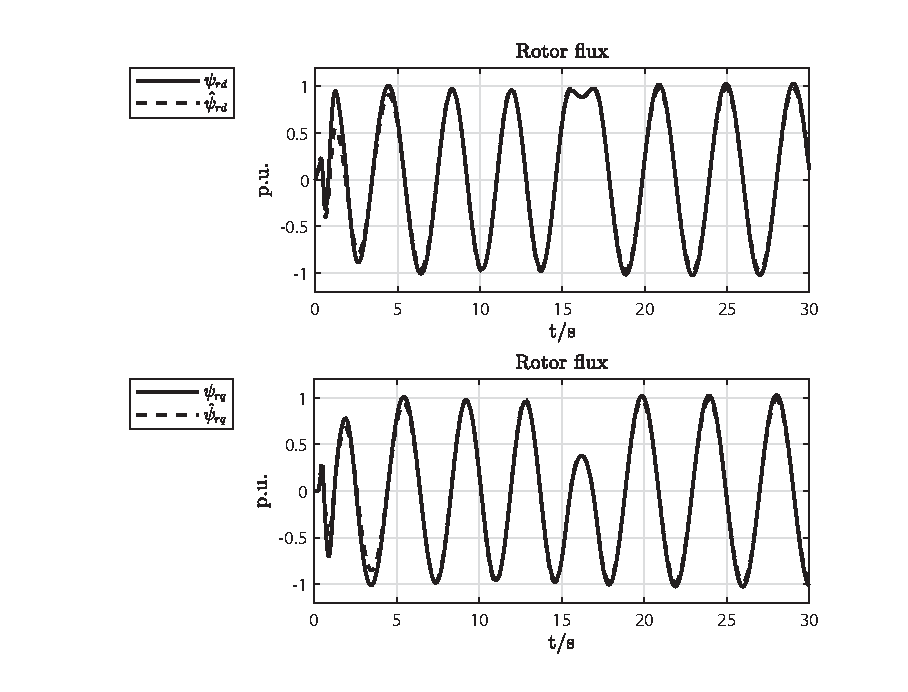
\includegraphics[width = 240pt, keepaspectratio]{figures/sim_results/cold_condition/rotor_flux_est_2.eps}
	\captionsetup{width=0.65\textwidth, font=footnotesize}	
	\caption{Estimated (dashed) and real (solid) rotor flux in $(d,q)$-(rotor frame) coordinates - $R_r^p > R_r$.}
	\label{fig_sim_res_20}
	\end{subfigure}		
	\captionsetup{width=0.5\textwidth, font=small}		
	\caption{Induction motor in cold condition.}
	\label{}
\end{figure}

\begin{figure}[H]
	\centering
	\begin{subfigure}{0.5\textwidth}
	\centering
	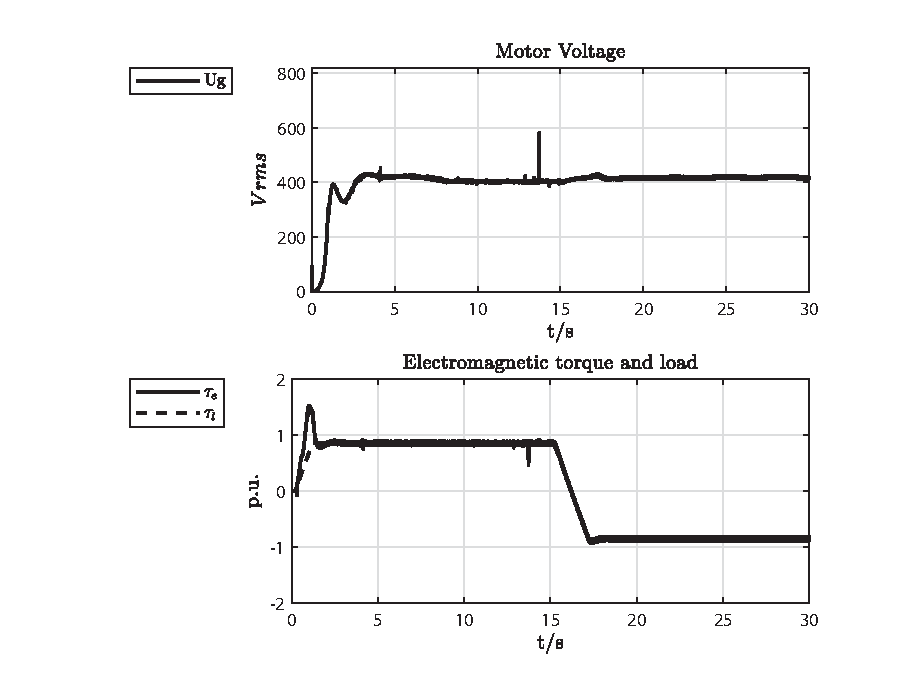
\includegraphics[width = 240pt, keepaspectratio]{figures/sim_results/cold_condition/motor_voltage.eps}
	\captionsetup{width=0.65\textwidth, font=footnotesize}	
	\caption{Motor voltage (phase to phase rms) and torques (electromagnetic and load) - $R_r^p > R_r$.}
	\label{fig_sim_res_21}
	\end{subfigure}%
	\begin{subfigure}{0.5\textwidth}
	\centering
	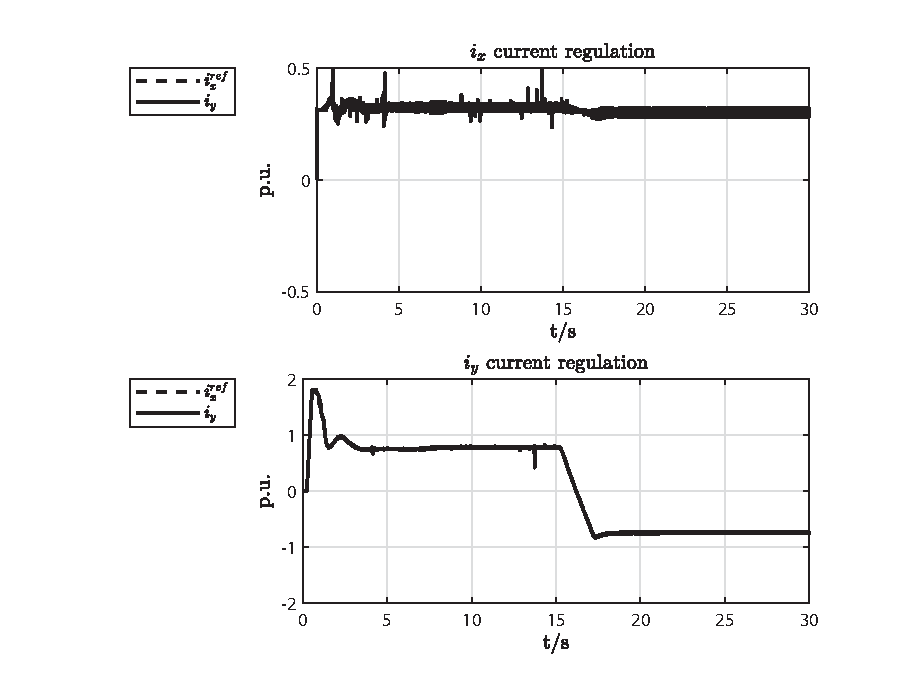
\includegraphics[width = 240pt, keepaspectratio]{figures/sim_results/cold_condition/current_reg.eps}
	\captionsetup{width=0.65\textwidth, font=footnotesize}	
	\caption{Stator current regulation in $(x,y)$ coordinates - synchronous reference frame - $R_r^p > R_r$.}
	\label{fig_sim_res_22}
	\end{subfigure}		
	\captionsetup{width=0.5\textwidth, font=small}	
	\caption{Induction motor in cold condition.}
	\label{}
\end{figure}

\begin{figure}[H]
	\centering
	\begin{subfigure}{0.5\textwidth}
	\centering
	\includegraphics[width = 240pt, keepaspectratio]{figures/sim_results/cold_condition/alpha_est.eps}
	\captionsetup{width=0.65\textwidth, font=footnotesize}		
	\caption{Rotor ${\alpha}$ estimation - $R_r^p > R_r$.}
	\label{fig_sim_res_23}
	\end{subfigure}%
	\begin{subfigure}{0.5\textwidth}
	\centering
	\includegraphics[width = 240pt, keepaspectratio]{figures/sim_results/cold_condition/current_obs.eps}
	\captionsetup{width=0.65\textwidth, font=footnotesize}		
	\caption{Stator current observer - $R_r^p > R_r$.}
	\label{fig_sim_res_24}
	\end{subfigure}		
	\captionsetup{width=0.5\textwidth, font=small}	
	\caption{Induction motor in cold condition.}
	\label{}
\end{figure}

\chapter{Appendices}

\section{Simscape Model: input/output and parameters}
The \textit{Simscape} model has been implemented by equation in machine variables according to section §~\ref{voltage_equations_in_machine_variables}.

The block model may be splitted into the following parts:
\begin{itemize}
	\item[--] physical node inputs;
	\item[--] physical signal outputs;
	\item[--] parameters.
\end{itemize} 

\noindent The \textbf{physical node inputs} consist of: 
\begin{itemize}
	\item[--] \texttt{S} [\SI{}{\radian\per\second}~--~\SI{}{\newton\meter}] : mechanical rotation node;
	\item[--] \texttt{uu\_p} [\SI{}{\volt}~--~\SI{}{\ampere}] : electrical u-positive pole;
	\item[--] \texttt{uv\_p} [\SI{}{\volt}~--~\SI{}{\ampere}] : electrical v-positive pole;
	\item[--] \texttt{uw\_p} [\SI{}{\volt}~--~\SI{}{\ampere}] : electrical w-positive pole;
	\item[--] \texttt{uu\_n} [\SI{}{\volt}~--~\SI{}{\ampere}] : electrical u-negative pole;
	\item[--] \texttt{uv\_n} [\SI{}{\volt}~--~\SI{}{\ampere}] : electrical v-negative pole;
	\item[--] \texttt{uw\_n} [\SI{}{\volt}~--~\SI{}{\ampere}] : electrical w-negative pole.
\end{itemize} 
For a star connection (Y-connection) the nodes \texttt{uu\_n}-\texttt{uv\_n}-\texttt{uw\_n} are connected together in a common floating center star (tap).

\noindent The \textbf{physical node inputs} consist of: 
\begin{itemize}
	\item[--] \texttt{is\_u} [\SI{}{\ampere}]: u-stator phase current;
	\item[--] \texttt{is\_v} [\SI{}{\ampere}]: v-stator phase current;
	\item[--] \texttt{is\_w} [\SI{}{\ampere}]: w-stator phase current;
	\item[--] \texttt{psi\_s\_u} [\SI{}{\volt\second}]: u-stator phase flux;
	\item[--] \texttt{psi\_s\_v} [\SI{}{\volt\second}]: v-stator phase flux;
	\item[--] \texttt{psi\_s\_w} [\SI{}{\volt\second}]: w-stator phase flux;
	\item[--] \texttt{psi\_r\_u} [\SI{}{\volt\second}]: u-rotor phase flux;
	\item[--] \texttt{psi\_r\_v} [\SI{}{\volt\second}]: v-rotor phase flux;
	\item[--] \texttt{psi\_r\_w} [\SI{}{\volt\second}]: w-rotor phase flux;
	\item[--] \texttt{tau\_e} [\SI{}{\newton\meter}]: electromagnetic torque;
	\item[--] \texttt{n} [\SI{}{\per\minute}]: mechanical rotational speed.
\end{itemize} 

\noindent The \textbf{motor parameters} consist of:
\begin{itemize}
	\item[--] \texttt{Lm} [\SI{}{\henry}]: mutual inductance between stator and rotor;
	\item[--] \texttt{Rs} [\SI{}{\ohm}]: stator per-phase electrical resistance;
	\item[--] \texttt{Lr} [\SI{}{\henry}]: rotor linkage inductance;
	\item[--] \texttt{Ls} [\SI{}{\henry}]: stator linkage inductance;
	\item[--] \texttt{Rr} [\SI{}{\ohm}]: rotor per-phase electrical resistance;
	\item[--] \texttt{J} [\SI{}{\kilogram\square\meter}]: rotor inertia;
	\item[--] \texttt{bm} [\SI{}{\newton\meter\second\per\radian}]: rotor friction;
	\item[--] \texttt{pole pairs} [--]: number of poles in the machine.
\end{itemize}

\begin{thebibliography}{99}

	\bibitem{krause}
	P. Krause, O. Wasynczuk, S. Sudhoff, S. Pekarek, \emph{Analysis of Electric Machinery and Drive Systems}. Wiley 2013.

	\bibitem{marino}
	R. Marino P. Tomei C.M. Verrelli, \emph{Induction Motor Control Desing}. Springer 2011.
			
	\bibitem{bianchi}
	N. Bianchi, T. Jahns, \emph{Design, analysis, and control of interior PM synchronous machines}. CLEUP 2004.

	\bibitem{umans}
	S.D. Umans, \emph{Fitzgerald \& Kingsley's Electric Machinery}. Mc Graw Hill 2014.
	
	\bibitem{khalil_1} 
	H.K. Khalil, \emph{Nonlinear Systems}. Third edition, Prentice Hall 
	2002.
	
	\bibitem{khalil_2} 
	H.K. Khalil, \emph{Nonlinear Control}. Pearson 2015.
	
	\bibitem{isidori} 
	A. Isidori, \emph{Nonlinear Control Systems}. Springer 1995.
	
	\bibitem{slotine} 
	J.J.E. Slotine, W. Li, \emph{Applied Nonlinear Control}. Prentice Hall 
	1991.

\end{thebibliography}
\end{document} 